\documentclass[12pt,a4paper,reqno]{amsart}
\usepackage[T1]{fontenc}
\usepackage[utf8]{inputenc}
\usepackage{lmodern,amsmath,amssymb,amsthm,microtype,enumitem,tasks,tikz,hyperref,needspace}
\newcommand{\krastineszymek}[1]{\tikz[baseline=(current bounding box.center)]{\foreach \x in {#1}{\draw (\x pt,-2.5pt)--(\x pt,2.5pt);}}}
\settasks{label-align=left,label-width=1.5em,label-offset=0.4em,item-indent=1.9em}
\emergencystretch=4em
\setlength{\parindent}{0pt}\setlength{\parskip}{0.6\baselineskip}
\makeatletter
\def\section{\@startsection{section}{1}{\z@}{-1.5\baselineskip plus -.3\baselineskip minus -.2\baselineskip}{0.6\baselineskip}{\normalfont\large\bfseries\raggedright}}
\makeatother
\theoremstyle{plain}\newtheorem{theorem}{Teorema}[section]
\newtheorem{lemma}[theorem]{Lema}\newtheorem{property}[theorem]{Savybė}\newtheorem{proposition}[theorem]{Teiginys}\newtheorem{corollary}[theorem]{Išvada}\newtheorem{conjecture}[theorem]{Hipotezė}
\theoremstyle{definition}
\newtheorem{definition}[theorem]{Apibrėžimas}\newtheorem{fact}[theorem]{Faktas}\newtheorem{example}[theorem]{Pavyzdys}\newtheorem{algorithm}[theorem]{Algoritmas}\newtheorem{question}[theorem]{Klausimas}\newtheorem{exercise}[theorem]{Pratimas}\newtheorem{problem}[theorem]{Uždavinys}\newtheorem{anchorproblem}[theorem]{Atraminis uždavinys}
\theoremstyle{remark}\newtheorem{remark}[theorem]{Pastaba}\newtheorem*{remark*}{Pastaba}
\theoremstyle{definition}\newtheorem*{problem*}{Uždavinys}
\newenvironment{starproblem}{\begingroup\let\numberwithoutstar\thetheorem\renewcommand{\thetheorem}{\numberwithoutstar\textsuperscript{*}}\begin{problem}}{\end{problem}\endgroup}
\newenvironment{staranchorproblem}{\begingroup\let\numberwithoutstar\thetheorem\renewcommand{\thetheorem}{\numberwithoutstar\textsuperscript{*}}\begin{anchorproblem}}{\end{anchorproblem}\endgroup}
\renewcommand{\proofname}{Įrodymas}\newenvironment{solution}[1][]{\par\medskip\Needspace{3\baselineskip}\noindent\textbf{#1.}\par\nobreak\noindent}{\par\medskip}
\newenvironment{answer}{\par\medskip\noindent\textit{Atsakymas.}\enspace}{\par\medskip}\newcommand{\ats}[1]{\par\noindent\textit{Atsakymas.} #1}
\newcommand{\kelias}[1]{\par\smallskip\noindent\textit{#1}\enspace}
\title[Trikampių lygumas]{Trikampių lygumas ir jo taikymai}
\newcommand{\poteme}{Antrasis temos karkaso variantas}
\author{Andrius Berniukevičius}\newcommand{\mokykla}{Vilniaus licėjus}
\makeatletter
\def\@settitle{\begin{center}{\large\bfseries \@title\par}\vspace{0.5em}{\normalsize\bfseries \poteme\par}\end{center}}
\def\@setauthors{\begin{center}\authors\par\vspace{0.3em}\mokykla\par\end{center}}
\makeatother\date{}
\begin{document}\maketitle
\section*{Įvadas}
Kaip iš kelių žinomų atkarpų ar kampų lygybių gauti naujų? Šiame lape mokysimės pasirinkti ir palyginti trikampius, o gautas išvadas taikysime kitiems uždaviniams.

Jau žinome du trikampių lygumo požymius: pagal dvi kraštines ir kampą tarp jų; pagal kraštinę ir du kampus prie jos. Taip pat žinome gretutinių ir kryžminių kampų savybes ir trikampio nelygybę: trikampis su kraštinėmis $a$, $b$, $c$ egzistuoja tada ir tik tada, kai kiekviena kraštinė mažesnė už kitų dviejų sumą. Remsimės ir įprastomis elementariosios geometrijos konstrukcijomis: atkarpos vidurio tašku, kampo pusiaukampine, kampo ir atkarpos atidėjimu (į nurodytą tiesės pusę tai galima padaryti vieninteliu būdu), taip pat tuo, kad per tašką galima nubrėžti vieną duotai tiesei statmeną tiesę. Šios konstrukcijos čia laikomos pradinėmis žiniomis. Paskutinįjį faktą tuo atveju, kai taškas nepriklauso tiesei, vėliau įrodysime (\ref{atr:statmuo} uždavinys).

Naudosimės ir akivaizdžiais taškų išsidėstymo faktais. Dvi skirtingos tiesės turi ne daugiau kaip vieną bendrą tašką. Jei taškas $B$ yra atkarpoje $AC$, tai $AC=AB+BC$. Atkarpa, jungianti taškus, esančius skirtingose tiesės pusėse, tą tiesę kerta. Sakome, kad spindulys $CD$ eina kampo $BCE$ viduje, jei taškas $D$ yra toje pačioje tiesės $CE$ pusėje kaip $B$ ir toje pačioje tiesės $CB$ pusėje kaip $E$. Tada $\angle BCE=\angle BCD+\angle DCE$, todėl kiekvienas iš kampų $BCD$ ir $DCE$ mažesnis už kampą $BCE$, o spindulys $CD$ kerta atkarpą $BE$.

Trikampio kampų sumos šiame dokumente nenaudojame. Žvaigždutė prie uždavinio numerio žymi sunkesnį uždavinį. Kai brėžinio nėra, nubraižykite jį patys.
\section{Lygumo įrodymo užrašymas}
Lygių trikampių atitinkamos kraštinės ir kampai lygūs. Užraše $\triangle ABC=\triangle DEF$ atitinka tose pačiose vietose esančios viršūnės: $A$ ir $D$, $B$ ir $E$, $C$ ir $F$. Šiame skyriuje lygius trikampius dar rasime brėžinyje; vėliau juos teks susikurti patiems.
\begin{problem}\label{uzd:breziniai-lygumas-01}
Kiekviename brėžinyje vienodais brūkšneliais pažymėtos atkarpos yra lygios, o vienodais lankeliais pažymėti kampai yra lygūs. Pažymėtas atkarpų susikirtimo taškas priklauso abiem atkarpoms. Remdamiesi šiais duomenimis, raskite po du lygius trikampius ir pagrįskite jų lygumą. Atkreipkite dėmesį į bendrus elementus ir kryžminius kampus: jie atskirai nepažymėti kaip lygūs, todėl paaiškinkite, kodėl jie lygūs. Naudokite tik du jau žinomus lygumo požymius. Pirmasis punktas – pavyzdys. Atitinkamas viršūnes užrašykite ta pačia tvarka.
\end{problem}
\par\medskip\Needspace{15\baselineskip}
\noindent\textbf{(1)}
\begin{center}
\begin{tikzpicture}[scale=0.9,baseline=(current bounding box.center)]
\coordinate (A) at (-1.85000,0.00000);
\coordinate (O) at (0.00000,0.00000);
\coordinate (C) at (1.85000,0.00000);
\coordinate (B) at (-0.80000,1.45000);
\coordinate (D) at (0.80000,-1.45000);
\draw (A)--(C);
\draw (B)--(D);
\draw (A)--(B);
\draw (C)--(D);
\node at ([shift={(-0.250cm,0.000cm)}]A) {$A$};
\node at ([shift={(0.250cm,0.000cm)}]C) {$C$};
\node at ([shift={(-0.080cm,0.240cm)}]B) {$B$};
\node at ([shift={(0.080cm,-0.240cm)}]D) {$D$};
\node at ([shift={(-0.180cm,-0.200cm)}]O) {$O$};
\path (A)--(O) node[midway,sloped,inner sep=0pt] {\krastineszymek{0}}
      (O)--(C) node[midway,sloped,inner sep=0pt] {\krastineszymek{0}};
\draw (-1.7034,0.2025) arc[start angle=54.0903,end angle=-0.0000,radius=0.250];
\draw (1.7034,-0.2025) arc[start angle=-125.9097,end angle=-180.0000,radius=0.250];
\end{tikzpicture}
\end{center}
Palyginkime trikampius $AOB$ ir $COD$:
\begin{itemize}[nosep]
\item $AO=CO$ (duota, pažymėta vienu brūkšneliu);
\item $\angle BAO=\angle DCO$ (duota, pažymėta vienu lankeliu);
\item $\angle AOB=\angle COD$ (kryžminiai kampai).
\end{itemize}
Lygūs kampai yra prie atitinkamai lygių kraštinių $AO$ ir $CO$. Todėl $\triangle AOB=\triangle COD$ pagal kraštinę ir du kampus prie jos.

\par\medskip\Needspace{15\baselineskip}
\noindent\textbf{(2)}
\begin{center}
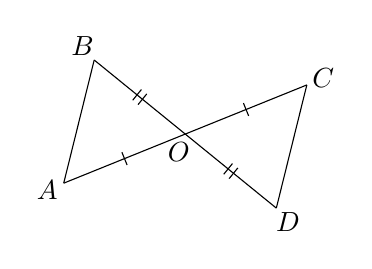
\begin{tikzpicture}[scale=0.9,baseline=(current bounding box.center)]
\coordinate (A) at (-1.71529,-0.69302);
\coordinate (O) at (0.00000,0.00000);
\coordinate (C) at (1.71529,0.69302);
\coordinate (B) at (-1.28493,1.04473);
\coordinate (D) at (1.28493,-1.04473);
\draw (A)--(C);
\draw (B)--(D);
\draw (A)--(B);
\draw (C)--(D);
\node at ([shift={(-0.232cm,-0.094cm)}]A) {$A$};
\node at ([shift={(0.232cm,0.094cm)}]C) {$C$};
\node at ([shift={(-0.164cm,0.193cm)}]B) {$B$};
\node at ([shift={(0.164cm,-0.193cm)}]D) {$D$};
\node at ([shift={(-0.092cm,-0.253cm)}]O) {$O$};
\path (A)--(O) node[midway,sloped,inner sep=0pt] {\krastineszymek{0}}
      (O)--(C) node[midway,sloped,inner sep=0pt] {\krastineszymek{0}}
      (B)--(O) node[midway,sloped,inner sep=0pt] {\krastineszymek{-1.25,1.25}}
      (O)--(D) node[midway,sloped,inner sep=0pt] {\krastineszymek{-1.25,1.25}};
\end{tikzpicture}
\end{center}
Palyginkime trikampius $\underline{\hspace{1.3cm}}$ ir $\underline{\hspace{1.3cm}}$:\par
\rule{0pt}{1.2em}\dotfill\par
\rule{0pt}{1.2em}\dotfill\par
\rule{0pt}{1.2em}\dotfill\par
Todėl $\triangle\underline{\hspace{1cm}}=\triangle\underline{\hspace{1cm}}$ pagal \dotfill .\par

\par\medskip\Needspace{15\baselineskip}
\noindent\textbf{(3)}
\begin{center}
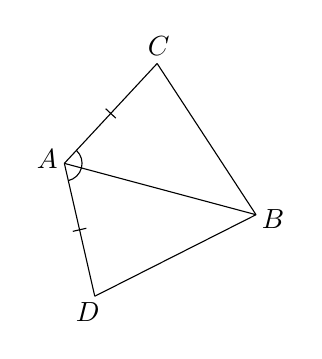
\begin{tikzpicture}[scale=0.9,baseline=(current bounding box.center)]
\coordinate (A) at (0.00000,0.00000);
\coordinate (B) at (2.70459,-0.72469);
\coordinate (C) at (1.30933,1.40914);
\coordinate (D) at (0.42934,-1.87501);
\draw (A)--(B);
\draw (A)--(C);
\draw (B)--(C);
\draw (A)--(D);
\draw (B)--(D);
\node at ([shift={(-0.241cm,0.065cm)}]A) {$A$};
\node at ([shift={(0.241cm,-0.065cm)}]B) {$B$};
\node at ([shift={(0.023cm,0.242cm)}]C) {$C$};
\node at ([shift={(-0.101cm,-0.221cm)}]D) {$D$};
\path (A)--(C) node[midway,sloped,inner sep=0pt] {\krastineszymek{0}}
      (A)--(D) node[midway,sloped,inner sep=0pt] {\krastineszymek{0}};
\draw (0.1702,0.1831) arc[start angle=47.1027,end angle=-15.0000,radius=0.250];
\draw (0.0558,-0.2437) arc[start angle=-77.1027,end angle=-15.0000,radius=0.250];
\end{tikzpicture}
\end{center}
Palyginkime trikampius $\underline{\hspace{1.3cm}}$ ir $\underline{\hspace{1.3cm}}$:\par
\rule{0pt}{1.2em}\dotfill\par
\rule{0pt}{1.2em}\dotfill\par
\rule{0pt}{1.2em}\dotfill\par
Todėl $\triangle\underline{\hspace{1cm}}=\triangle\underline{\hspace{1cm}}$ pagal \dotfill .\par

\par\medskip\Needspace{15\baselineskip}
\noindent\textbf{(4)}
\begin{center}
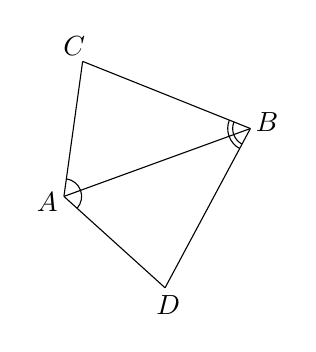
\begin{tikzpicture}[scale=0.9,baseline=(current bounding box.center)]
\coordinate (A) at (0.00000,0.00000);
\coordinate (B) at (2.63114,0.95766);
\coordinate (C) at (0.26429,1.90530);
\coordinate (D) at (1.42716,-1.28966);
\draw (A)--(B);
\draw (A)--(C);
\draw (B)--(C);
\draw (A)--(D);
\draw (B)--(D);
\node at ([shift={(-0.235cm,-0.086cm)}]A) {$A$};
\node at ([shift={(0.235cm,0.086cm)}]B) {$B$};
\node at ([shift={(-0.120cm,0.212cm)}]C) {$C$};
\node at ([shift={(0.044cm,-0.239cm)}]D) {$D$};
\draw (0.0343,0.2476) arc[start angle=82.1027,end angle=20.0000,radius=0.250];
\draw (0.1855,-0.1676) arc[start angle=-42.1027,end angle=20.0000,radius=0.250];
\draw (2.3962,0.8722) arc[start angle=-160.0000,end angle=-201.8202,radius=0.250];
\draw (2.3304,0.8482) arc[start angle=-160.0000,end angle=-201.8202,radius=0.320];
\draw (2.3962,0.8722) arc[start angle=-160.0000,end angle=-118.1798,radius=0.250];
\draw (2.3304,0.8482) arc[start angle=-160.0000,end angle=-118.1798,radius=0.320];
\end{tikzpicture}
\end{center}
Įrodymas:\par
\rule{0pt}{1.2em}\dotfill\par
\rule{0pt}{1.2em}\dotfill\par
\rule{0pt}{1.2em}\dotfill\par
\rule{0pt}{1.2em}\dotfill\par
\rule{0pt}{1.2em}\dotfill\par

\par\medskip\Needspace{15\baselineskip}
\noindent\textbf{(5)}
\begin{center}
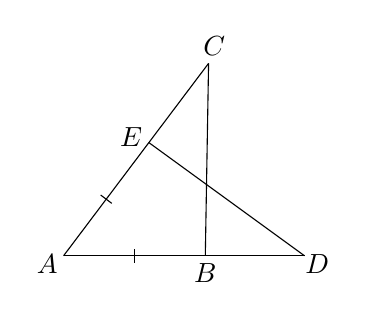
\begin{tikzpicture}[scale=0.9,baseline=(current bounding box.center)]
\coordinate (A) at (0.00000,0.00000);
\coordinate (B) at (2.00000,0.00000);
\coordinate (D) at (3.40000,0.00000);
\coordinate (C) at (2.04617,2.71536);
\coordinate (E) at (1.20363,1.59727);
\draw (A)--(D);
\draw (A)--(C);
\draw (B)--(C);
\draw (D)--(E);
\node at ([shift={(-0.230cm,-0.120cm)}]A) {$A$};
\node at ([shift={(0.000cm,-0.250cm)}]B) {$B$};
\node at ([shift={(0.180cm,-0.120cm)}]D) {$D$};
\node at ([shift={(0.080cm,0.240cm)}]C) {$C$};
\node at ([shift={(-0.250cm,0.080cm)}]E) {$E$};
\path (A)--(B) node[midway,sloped,inner sep=0pt] {\krastineszymek{0}}
      (A)--(E) node[midway,sloped,inner sep=0pt] {\krastineszymek{0}};
\end{tikzpicture}
\end{center}
Duota: $AB=AE$ ir $AC=AD$.

Įrodymas:\par
\rule{0pt}{1.2em}\dotfill\par
\rule{0pt}{1.2em}\dotfill\par
\rule{0pt}{1.2em}\dotfill\par
\rule{0pt}{1.2em}\dotfill\par
\rule{0pt}{1.2em}\dotfill\par


\begin{problem}\label{uzd:lygybe-atitikimas-01} Žinoma, kad $\triangle ABC=\triangle PQR$. Kurios kraštinės atitinka $AB$ ir $AC$? Kurie kampai atitinka $\angle ABC$ ir $\angle BAC$? Užrašykite likusių atitinkamų kraštinių ir kampų lygybes. \end{problem}
\begin{problem}\label{uzd:lygybe-sas-01} Duota $AB=FE$, $AC=FD$, $\angle BAC=\angle EFD$. Įrodykite, kad trikampiai $ABC$ ir $FED$ lygūs. Kuri kraštinė lygi $BC$? \end{problem}
\begin{problem}\label{uzd:lygybe-asa-01} Trikampiuose $ABC$ ir $KLM$ žinoma: $AB=KL$, $\angle BAC=\angle LKM$, $\angle ABC=\angle KLM$. Įrodykite, kad trikampiai lygūs, ir nurodykite $AC$ atitinkančią kraštinę. \end{problem}
\begin{problem}\label{uzd:lygybe-klaida-01} Mokinys tvirtina: „Jeigu $AB=DE$, $AC=DF$ ir $\angle ABC=\angle DEF$, tai trikampiai lygūs pagal dvi kraštines ir kampą tarp jų.“ Paaiškinkite, kodėl nurodytu požymiu taip remtis negalima. Ar užtektų papildomos sąlygos $\angle BAC=\angle EDF$? \end{problem}
\begin{problem}\label{uzd:lygybe-ssa-01} Ar iš dviejų kraštinių ir kampo, kuris nėra tarp jų, lygybės išplaukia trikampių lygumas? Ištirkite tokį pavyzdį. Pasirinkite taškus $A$, $C$, $D$, nesančius vienoje tiesėje, taip, kad $AC=AD$, ir pratęskite atkarpą $CD$ už taško $D$ iki taško $B$. Kurios trikampių $ABC$ ir $ABD$ kraštinės ir kampai lygūs? Ar šie trikampiai lygūs? \end{problem}
\begin{center}
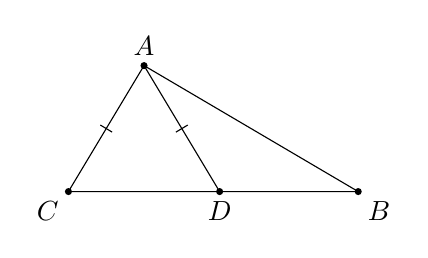
\begin{tikzpicture}[scale=.8]
\coordinate (A) at (1.2,2);\coordinate (C) at (0,0);\coordinate (D) at (2.4,0);\coordinate (B) at (4.6,0);
\draw (C)--(B) (A)--(C) (A)--(D) (A)--(B);
\path (A)--(C) node[midway,sloped,inner sep=0pt] {\krastineszymek{0}}
      (A)--(D) node[midway,sloped,inner sep=0pt] {\krastineszymek{0}};
\foreach \p/\pos in {A/above,C/below left,D/below,B/below right} {\fill (\p) circle (1.6pt) node[\pos] {$\p$};}
\end{tikzpicture}
\end{center}
\begin{problem}\label{uzd:lygybe-susikirtimas-01} Atkarpos $AC$ ir $BD$ kertasi taške $O$. Duota $AO=OC$ ir $BO=OD$. Įrodykite, kad $AB=CD$ ir $AD=CB$. Raskite dar dvi lygių trikampių poras, kurių viršūnė nėra taškas $O$, ir pagrįskite jų lygumą. \end{problem}
\begin{center}
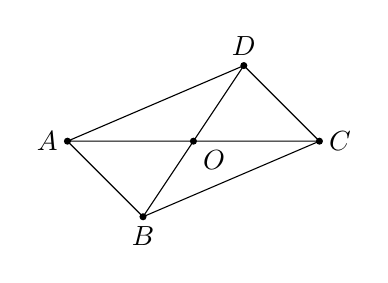
\begin{tikzpicture}[scale=0.8]
\coordinate (O) at (0,0); \coordinate (A) at (-2,0); \coordinate (C) at (2,0); \coordinate (B) at (-.8,-1.2); \coordinate (D) at (.8,1.2);
\draw (A)--(C) (B)--(D) (A)--(B) (C)--(D) (A)--(D) (B)--(C);
\foreach \p/\pos in {A/left,B/below,D/above,C/right,O/below right} {\fill (\p) circle (1.6pt) node[\pos] {$\p$};}
\end{tikzpicture}
\end{center}
\begin{problem}\label{uzd:lygybe-pusiaukampine-01} Taškas $D$ yra trikampio $ABC$ kraštinėje $BC$, $AB=AC$, o $AD$ yra kampo $BAC$ pusiaukampinė. Įrodykite, kad $BD=DC$ ir $AD\perp BC$. \end{problem}
\section{Lygiašonis trikampis}
\kelias{Kur einame.} Iki šiol lygius trikampius radome brėžinyje. Dabar patys nuspręsime, kokią liniją nubrėžti, kad atsirastų du lygūs trikampiai: lygiašoniame trikampyje tokia linija yra pusiaukampinė iš viršūnės. Atkreipkite dėmesį ir į kitą gudrybę: trikampį galima palyginti su juo pačiu, tik viršūnes surašius kita tvarka (\ref{atr:lygias-atvirkstine} uždavinys).
\Needspace{10\baselineskip}
\begin{definition}\label{apib:lygias-trikampis} Trikampis, kurio dvi kraštinės lygios, vadinamas \emph{lygiašoniu}. Šios kraštinės vadinamos šoninėmis, o trečioji – pagrindu.
\begin{center}
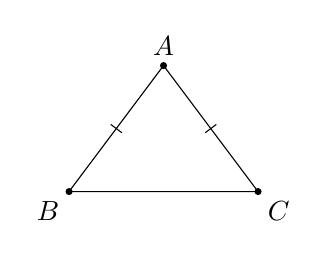
\begin{tikzpicture}[scale=.8]
\coordinate (A) at (1.5,2);\coordinate (B) at (0,0);\coordinate (C) at (3,0);
\draw (A)--(B) node[midway,sloped,inner sep=0pt] {\krastineszymek{0}}--(C)--(A) node[midway,sloped,inner sep=0pt] {\krastineszymek{0}};
\foreach \p/\pos in {A/above,B/below left,C/below right} {\fill (\p) circle (1.6pt) node[\pos] {$\p$};}
\end{tikzpicture}
\end{center}
\end{definition}
\begin{problem}\label{uzd:lygias-supratimas-01} Trikampyje $ABC$ duota $AB=AC$. Nurodykite pagrindą ir kampus prie pagrindo. Ar trikampis, kurio visos kraštinės lygios, atitinka apibrėžimą? Ar galima pasirinkti bet kurią jo kraštinę pagrindu? \end{problem}
\begin{starproblem}\label{uzd:lygias-perimetras-01} Lygiašonio trikampio perimetras yra $20$ cm, o viena kraštinė lygi $6$ cm. Raskite likusių dviejų kraštinių ilgius. \end{starproblem}
\begin{anchorproblem}[Lygiašonio trikampio kampų prie pagrindo savybė]\label{atr:lygias-pagrindo-kampai} Nubrėžkite lygiašonio trikampio kampo tarp šoninių kraštinių pusiaukampinę ir įrodykite, kad kampai prie pagrindo lygūs. \end{anchorproblem}
\begin{problem}\label{uzd:lygias-kampai-01} Trikampyje $ABC$ duota $AB=AC$. Raskite $\angle ACB$, jei $\angle ABC=38^\circ$. Ar iš šių duomenų išplaukia, kad $AB=BC$? \end{problem}
\begin{problem}\label{uzd:lygias-kampai-02} Trikampyje $PQR$ duota $PQ=QR$, $\angle QPR=2x+10^\circ$, $\angle PRQ=3x-5^\circ$. Raskite $x$ ir abu nurodytus kampus. \end{problem}
\begin{anchorproblem}[Lygiašonio trikampio požymis]\label{atr:lygias-atvirkstine} Įrodykite: jei du trikampio kampai lygūs, tai prieš juos esančios kraštinės lygios. \end{anchorproblem}
\begin{problem}\label{uzd:lygias-atvirkstine-01} Trikampyje $ABC$ žinoma, kad $\angle ABC=\angle BCA$ ir $AB=7$ cm. Raskite $AC$. \end{problem}
\begin{problem}\label{uzd:lygias-atvirkstine-02} Trikampyje $KLM$ žinoma, kad $\angle KLM=\angle LKM$. Kurios dvi trikampio kraštinės lygios? Paaiškinkite, kodėl kampai $K$ ir $M$ nebūtinai lygūs. \end{problem}
\begin{anchorproblem}\label{atr:lygias-pusiaukrastine} Trikampyje $ABC$ duota $AB=AC$, o $M$ yra $BC$ vidurio taškas. Įrodykite, kad pusiaukraštinė $AM$ yra ir aukštinė, ir kampo $BAC$ pusiaukampinė. \end{anchorproblem}
\begin{problem}\label{uzd:lygias-pusiaukrastine-01} Trikampyje $ABC$ duota $AB=AC$, $BM=MC$ ir $\angle BAM=27^\circ$. Raskite $\angle MAC$ ir $\angle AMB$. \end{problem}
\begin{problem}\label{uzd:lygias-aukstine-01} Trikampyje $ABC$ duota $AB=AC$, $D$ yra kraštinėje $BC$ ir $AD\perp BC$. Įrodykite, kad $BD=DC$ ir $\angle BAD=\angle DAC$. \end{problem}
\begin{problem}\label{uzd:lygias-pusiaukampines-01} Trikampyje $ABC$ duota $AB=AC$. Kampų $ABC$ ir $ACB$ pusiaukampinės kerta kraštines $AC$ ir $AB$ atitinkamai taškuose $D$ ir $E$. Įrodykite, kad $BD=CE$. \end{problem}
\Needspace{10\baselineskip}
\begin{definition}\label{apib:lygiakrastis} Trikampis, kurio visos trys kraštinės lygios, vadinamas \emph{lygiakraščiu}.
\begin{center}
\begin{tikzpicture}[scale=.8]
\coordinate (A) at (1.5,2.59808);\coordinate (B) at (0,0);\coordinate (C) at (3,0);
\draw (A)--(B) node[midway,sloped,inner sep=0pt] {\krastineszymek{0}}--(C) node[midway,sloped,inner sep=0pt] {\krastineszymek{0}}--(A) node[midway,sloped,inner sep=0pt] {\krastineszymek{0}};
\foreach \p/\pos in {A/above,B/below left,C/below right} {\fill (\p) circle (1.6pt) node[\pos] {$\p$};}
\end{tikzpicture}
\end{center}
\end{definition}
\begin{problem}\label{uzd:lygiakrastis-supratimas-01} Ar kiekvienas lygiakraštis trikampis yra lygiašonis? Ar kiekvienas lygiašonis yra lygiakraštis? Pateikite pavyzdį arba paaiškinkite. \end{problem}
\begin{anchorproblem}[Lygiakraščio trikampio savybė ir požymis]\label{atr:lygiakrastis-kampai} Įrodykite: lygiakraščio trikampio visi kampai lygūs; jei visi trikampio kampai lygūs, tai trikampis lygiakraštis. \end{anchorproblem}
\begin{problem}\label{uzd:lygiakrastis-kampai-01} Trikampyje $ABC$ duota $AB=BC=CA$. Palyginkite $\angle BAC$ ir $\angle BCA$. Ar iš čia galima teigti, kad abu šie kampai yra po $60^\circ$, nepasitelkus papildomo fakto? \end{problem}
\section{Trečiasis trikampių lygumo požymis}
\kelias{Kur einame.} Abiem žinomiems požymiams reikėjo kampų. Ar trikampį nusako vien jo kraštinės? Įrodymo idėja tokia: du trikampius sustatome taip, kad susidarytų du lygiašoniai trikampiai su bendru pagrindu, ir pasiremiame jų kampais prie pagrindo. Šį derinį vėl sutiksime vidurio statmens skyriuje. Įrodyme teks nagrinėti kelis taškų išsidėstymo atvejus: brėžinys rodo tik vieną iš jų.
\begin{staranchorproblem}[Trikampių lygumo požymis pagal tris kraštines]\label{atr:sss-poz}

Duoti trikampiai $ABC$ ir $DEF$, kurių $AB=DF$, $BC=FE$ ir $AC=DE$. Lygios kraštinės pažymėtos vienodu brūkšnelių skaičiumi. Įrodysime, kad šie trikampiai lygūs.
\begin{center}
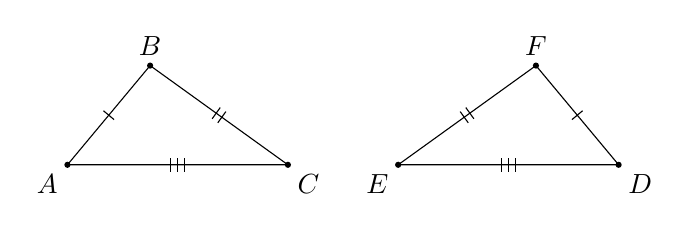
\begin{tikzpicture}[scale=.7]
\coordinate (A) at (0,0);\coordinate (B) at (1.5,1.8);\coordinate (C) at (4,0);
\coordinate (D) at (10,0);\coordinate (F) at (8.5,1.8);\coordinate (E) at (6,0);
\draw (A)--(B) node[midway,sloped,inner sep=0pt] {\krastineszymek{0}}--(C) node[midway,sloped,inner sep=0pt] {\krastineszymek{-1.25,1.25}}--(A) node[midway,sloped,inner sep=0pt] {\krastineszymek{-2.5,0,2.5}};
\draw (D)--(F) node[midway,sloped,inner sep=0pt] {\krastineszymek{0}}--(E) node[midway,sloped,inner sep=0pt] {\krastineszymek{-1.25,1.25}}--(D) node[midway,sloped,inner sep=0pt] {\krastineszymek{-2.5,0,2.5}};
\foreach \p/\pos in {A/below left,B/above,C/below right,D/below right,F/above,E/below left}
{\fill (\p) circle (1.6pt) node[\pos] {$\p$};}
\end{tikzpicture}
\end{center}
\begin{enumerate}[label=\alph*),leftmargin=*]
\item Kitoje tiesės $AC$ pusėje nei taškas $B$ atidėkite kampą $CAK$, lygų kampui $EDF$, o jo kraštinėje – atkarpą $AK=DF$. Nubrėžkite atkarpas $KC$ ir $BK$. Įrodykite, kad $\triangle AKC=\triangle DFE$, ir iš čia išveskite, kad $AK=AB$ ir $CK=CB$.
\begin{center}
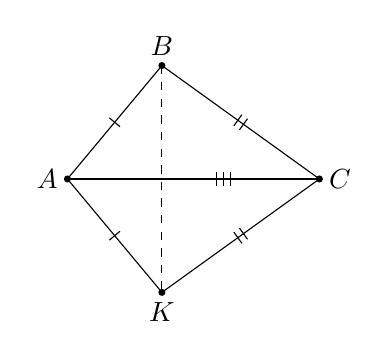
\begin{tikzpicture}[scale=.8]
\coordinate (A) at (0,0);\coordinate (B) at (1.5,1.8);\coordinate (C) at (4,0);\coordinate (K) at (1.5,-1.8);
\draw (A)--(B) node[midway,sloped,inner sep=0pt] {\krastineszymek{0}}--(C) node[midway,sloped,inner sep=0pt] {\krastineszymek{-1.25,1.25}}--(K) node[midway,sloped,inner sep=0pt] {\krastineszymek{-1.25,1.25}}--(A) node[midway,sloped,inner sep=0pt] {\krastineszymek{0}};
\draw (A)--(C) node[pos=.62,sloped,inner sep=0pt] {\krastineszymek{-2.5,0,2.5}};
\draw[dashed] (B)--(K);
\foreach \p/\pos in {A/left,B/above,C/right,K/below}
{\fill (\p) circle (1.6pt) node[\pos] {$\p$};}
\end{tikzpicture}
\end{center}
\item Taškai $B$ ir $K$ yra skirtingose tiesės $AC$ pusėse, todėl atkarpa $BK$ kerta šią tiesę; sankirtos tašką pažymėkite $X$. Įrodykite, kad $\angle ABC=\angle AKC$, atskirai išnagrinėdami tris atvejus: $X$ yra tarp $A$ ir $C$; $X$ sutampa su $A$ arba su $C$; $X$ yra už atkarpos $AC$.
\begin{center}
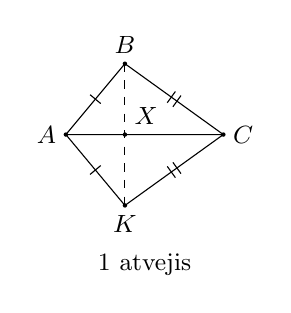
\begin{tikzpicture}[scale=.5,font=\small]
\coordinate (A) at (0,0);\coordinate (C) at (4,0);\coordinate (B) at (1.5,1.8);\coordinate (K) at (1.5,-1.8);\coordinate (X) at (1.5,0);
\draw (A)--(B)--(C)--(K)--cycle (A)--(C);
\draw[dashed] (B)--(K);
\path (A)--(B) node[midway,sloped,inner sep=0pt] {\krastineszymek{0}}
      (A)--(K) node[midway,sloped,inner sep=0pt] {\krastineszymek{0}}
      (B)--(C) node[midway,sloped,inner sep=0pt] {\krastineszymek{-1.25,1.25}}
      (K)--(C) node[midway,sloped,inner sep=0pt] {\krastineszymek{-1.25,1.25}};
\foreach \p/\pos in {A/left,B/above,C/right,K/below,X/above right} {\fill (\p) circle (1.6pt) node[\pos] {$\p$};}
\node at (2,-3.3) {1 atvejis};
\end{tikzpicture}\hspace{1.2em}
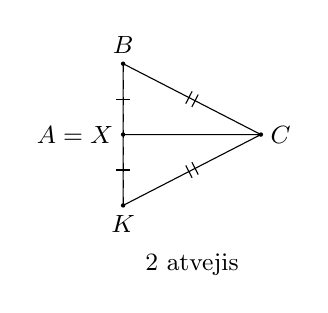
\begin{tikzpicture}[scale=.5,font=\small]
\coordinate (A) at (0,0);\coordinate (C) at (3.5,0);\coordinate (B) at (0,1.8);\coordinate (K) at (0,-1.8);
\draw (A)--(B)--(C)--(K)--cycle (A)--(C);
\draw[dashed] (B)--(K);
\path (A)--(B) node[midway,sloped,inner sep=0pt] {\krastineszymek{0}}
      (A)--(K) node[midway,sloped,inner sep=0pt] {\krastineszymek{0}}
      (B)--(C) node[midway,sloped,inner sep=0pt] {\krastineszymek{-1.25,1.25}}
      (K)--(C) node[midway,sloped,inner sep=0pt] {\krastineszymek{-1.25,1.25}};
\foreach \p/\pos in {B/above,C/right,K/below} {\fill (\p) circle (1.6pt) node[\pos] {$\p$};}
\fill (A) circle (1.6pt) node[left] {$A=X$};
\node at (1.75,-3.3) {2 atvejis};
\end{tikzpicture}\hspace{1.2em}
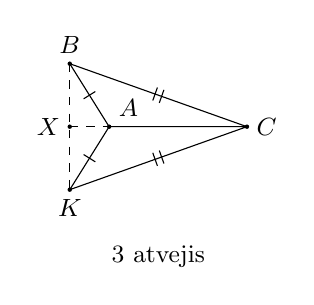
\begin{tikzpicture}[scale=.5,font=\small]
\coordinate (A) at (0,0);\coordinate (C) at (3.5,0);\coordinate (B) at (-1,1.6);\coordinate (K) at (-1,-1.6);\coordinate (X) at (-1,0);
\draw (A)--(B)--(C)--(K)--cycle (A)--(C);
\draw[dashed] (B)--(K) (X)--(A);
\path (A)--(B) node[midway,sloped,inner sep=0pt] {\krastineszymek{0}}
      (A)--(K) node[midway,sloped,inner sep=0pt] {\krastineszymek{0}}
      (B)--(C) node[midway,sloped,inner sep=0pt] {\krastineszymek{-1.25,1.25}}
      (K)--(C) node[midway,sloped,inner sep=0pt] {\krastineszymek{-1.25,1.25}};
\foreach \p/\pos in {A/above right,B/above,C/right,K/below,X/left} {\fill (\p) circle (1.6pt) node[\pos] {$\p$};}
\node at (1.25,-3.3) {3 atvejis};
\end{tikzpicture}
\end{center}
\item Įrodykite, kad $\triangle ABC=\triangle AKC$, ir išveskite, kad $\triangle ABC=\triangle DFE$. Lygybę užrašykite nurodydami atitinkamas viršūnes ta pačia tvarka.
\end{enumerate}
\end{staranchorproblem}
\begin{problem}\label{uzd:sss-breziniai-01}
Kiekviename brėžinyje raskite du lygius trikampius ir pagrįskite jų lygumą pagal tris kraštines. Atitinkamas viršūnes užrašykite ta pačia tvarka.
\begin{tasks}(1)
\task $AB=AD$, $CB=CD$.
\begin{center}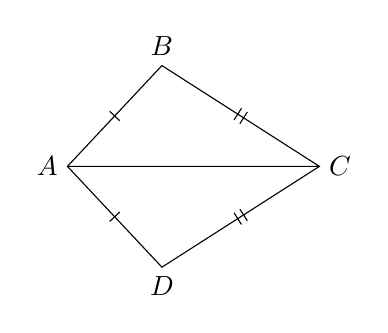
\begin{tikzpicture}[scale=.8]
\coordinate (A) at (0,0);\coordinate (C) at (4,0);\coordinate (B) at (1.5,1.6);\coordinate (D) at (1.5,-1.6);
\draw (A)--(B)--(C)--(D)--cycle (A)--(C);
\path (A)--(B) node[midway,sloped,inner sep=0pt] {\krastineszymek{0}}
      (A)--(D) node[midway,sloped,inner sep=0pt] {\krastineszymek{0}}
      (C)--(B) node[midway,sloped,inner sep=0pt] {\krastineszymek{-1.25,1.25}}
      (C)--(D) node[midway,sloped,inner sep=0pt] {\krastineszymek{-1.25,1.25}};
\foreach \p/\d in {A/left,B/above,C/right,D/below} \node[\d] at (\p) {$\p$};
\end{tikzpicture}\end{center}
\task Taškai $A,B,D$ yra vienoje tiesėje, $B$ yra tarp $A$ ir $D$; taškai $A,E,C$ yra vienoje tiesėje, $E$ yra tarp $A$ ir $C$. Duota $AB=AE$, $AC=AD$ ir $BC=DE$. Ar duomuo $BC=DE$ būtinas? Įrodykite trikampių lygumą juo nesinaudodami.
\begin{center}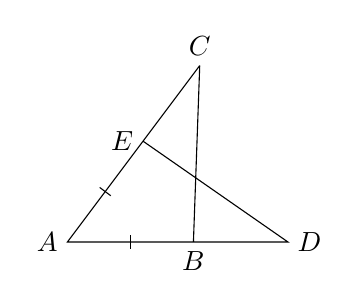
\begin{tikzpicture}[scale=.8]
\coordinate (A) at (0,0);\coordinate (B) at (2,0);\coordinate (D) at (3.5,0);\coordinate (E) at (1.2,1.6);\coordinate (C) at (2.1,2.8);
\draw (A)--(D)--(E)--(C)--cycle (B)--(C);
\path (A)--(B) node[midway,sloped,inner sep=0pt] {\krastineszymek{0}}
      (A)--(E) node[midway,sloped,inner sep=0pt] {\krastineszymek{0}};
\foreach \p/\d in {A/left,B/below,D/right,E/left,C/above} \node[\d] at (\p) {$\p$};
\end{tikzpicture}\end{center}
\task Taškai $A,B,C$ yra vienoje tiesėje, o $D,E,F$ – kitoje; $B$ yra tarp $A$ ir $C$, $E$ – tarp $D$ ir $F$. Duota $AB=DE$, $BC=EF$, $AG=DG$ ir $CG=FG$.
\begin{center}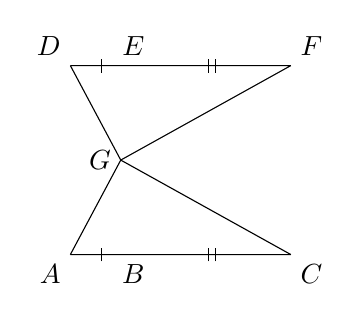
\begin{tikzpicture}[scale=.8]
\coordinate (A) at (0,0);\coordinate (B) at (1,0);\coordinate (C) at (3.5,0);\coordinate (D) at (0,3);\coordinate (E) at (1,3);\coordinate (F) at (3.5,3);\coordinate (G) at (.8,1.5);
\draw (A)--(C) (D)--(F) (A)--(G)--(C) (D)--(G)--(F);
\path (A)--(B) node[midway,sloped,inner sep=0pt] {\krastineszymek{0}}
      (D)--(E) node[midway,sloped,inner sep=0pt] {\krastineszymek{0}}
      (B)--(C) node[midway,sloped,inner sep=0pt] {\krastineszymek{-1.25,1.25}}
      (E)--(F) node[midway,sloped,inner sep=0pt] {\krastineszymek{-1.25,1.25}};
\foreach \p/\d in {A/below left,B/below,C/below right,D/above left,E/above,F/above right,G/left} \node[\d] at (\p) {$\p$};
\end{tikzpicture}\end{center}
\end{tasks}
\end{problem}

\begin{problem}\label{uzd:sss-tiesioginis-01} Duota $AB=PR$, $BC=RQ$, $CA=QP$. Užrašykite trikampių $ABC$ ir $PQR$ lygumą taip, kad viršūnės atitiktų, ir nurodykite požymį. \end{problem}
\begin{problem}\label{uzd:sss-tiesioginis-02} Atkarpos $AC$ ir $BD$ kertasi taške $O$. Duota $AB=CD$ ir $AD=CB$. Įrodykite, kad $\angle BAD=\angle DCB$, $\angle ABD=\angle CDB$ ir $\angle ADB=\angle CBD$. \end{problem}
\begin{remark*} Kai išmoksime lygiagrečių tiesių požymius, iš paskutinių dviejų lygybių gausime $AB\parallel CD$ ir $AD\parallel BC$. Tai bus lygiagretainio požymių pagrindas. \end{remark*}
\begin{starproblem}\label{uzd:sss-konstr-01} Nubraižykite atkarpą $AB$ ir tašką $C$, nepriklausantį tiesei $AB$. Kitoje tiesės $AB$ pusėje skriestuvu raskite tašką $D$, kuriam $AD=AC$, $BD=BC$. Pagrįskite, kad toks taškas egzistuoja ir kad $\triangle ABC=\triangle ABD$. Kiek tokių taškų $D$ gali būti toje pusėje? \end{starproblem}
\section{Trikampio priekampis}
\kelias{Kur einame.} Iki šiol įrodinėjome tik lygybes. Dabar pirmą kartą įrodysime kampų nelygybę. Pagrindinis įrankis – \emph{pusiaukraštinės pratęsimas dvigubai}: pratęsę pusiaukraštinę už kraštinės vidurio tiek pat, gauname naują trikampį, lygų vienai pradinio trikampio daliai, ir taip „perkeliame“ kampą į kitą vietą. Šį metodą dar panaudosime \ref{uzd:priekampis-pusiaukrastine} uždavinyje.
\Needspace{10\baselineskip}
\begin{definition}\label{apib:priekampis} Trikampio \emph{priekampis} yra kampas, gretutinis trikampio vidaus kampui. Pavyzdžiui, jei taškas $E$ yra tiesėje $AC$ už taško $C$, tai $\angle BCE$ yra trikampio $ABC$ priekampis prie viršūnės $C$.
\begin{center}
\begin{tikzpicture}[scale=.8]
\coordinate (A) at (-2,0);\coordinate (B) at (0,2);\coordinate (C) at (2,0);\coordinate (E) at (4.7,0);
\draw (A)--(E) (A)--(B)--(C);
\draw (2.5,0) arc[start angle=0,end angle=135,radius=.5];
\foreach \p/\pos in {A/left,B/above,C/below,E/right} {\fill (\p) circle (1.6pt) node[\pos] {$\p$};}
\end{tikzpicture}
\end{center}
\end{definition}
\begin{problem}\label{uzd:priekampis-supratimas} Nubrėžkite trikampį $ABC$, pratęskite $AC$ už $C$ ir pažymėkite priekampį. Kuris trikampio kampas yra jam gretutinis? Kurie du trikampio kampai nėra jam gretutiniai? \end{problem}
\begin{staranchorproblem}[Trikampio priekampio nelygybė]\label{atr:priekampis-nelygybe}
Duotas trikampis $ABC$ ir jo priekampis $BCE$: kraštinė $AC$ pratęsta už viršūnės $C$ iki taško $E$. Įrodykite, kad šis priekampis didesnis už kiekvieną jam negretutinį trikampio kampą.
\begin{center}
\begin{tikzpicture}[scale=.8]
\coordinate (A) at (-2,0);\coordinate (B) at (0,2);\coordinate (C) at (2,0);\coordinate (E) at (4.7,0);
\draw (A)--(E) (A)--(B)--(C);
\foreach \p/\pos in {A/left,B/above,C/below,E/right} {\fill (\p) circle (1.6pt);\node[\pos] at (\p) {$\p$};}
\end{tikzpicture}
\end{center}
\begin{enumerate}[label=\alph*),leftmargin=*]
\item Pažymėkite kraštinės $BC$ vidurio tašką $M$. Pratęskite atkarpą $AM$ už $M$ iki taško $D$ taip, kad $MD=MA$, ir nubrėžkite $CD$, kaip parodyta brėžinyje. Įrodykite, kad $\triangle ABM=\triangle DCM$.
\begin{center}
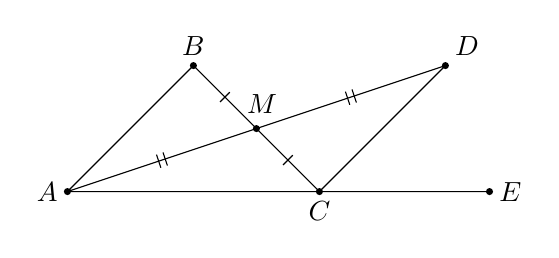
\begin{tikzpicture}[scale=.8]
\coordinate (A) at (-2,0);\coordinate (B) at (0,2);\coordinate (C) at (2,0);\coordinate (E) at (4.7,0);\coordinate (M) at (1,1);\coordinate (D) at (4,2);
\draw (A)--(E) (A)--(B)--(C)--(D) (A)--(D);
\path (B)--(M) node[midway,sloped,inner sep=0pt] {\krastineszymek{0}}
      (M)--(C) node[midway,sloped,inner sep=0pt] {\krastineszymek{0}}
      (A)--(M) node[midway,sloped,inner sep=0pt] {\krastineszymek{-1.25,1.25}}
      (M)--(D) node[midway,sloped,inner sep=0pt] {\krastineszymek{-1.25,1.25}};
\foreach \p/\pos in {A/left,B/above,C/below,E/right,D/above right} {\fill (\p) circle (1.6pt);\node[\pos] at (\p) {$\p$};}
\fill (M) circle (1.6pt) node[above=2pt,xshift=2pt] {$M$};
\end{tikzpicture}
\end{center}
\item Įrodykite, kad spindulys $CD$ eina kampo $BCE$ viduje, ir išveskite, kad $\angle BCE>\angle ABC$.
\item Panašią konstrukciją atlikite su kraštine $AC$: naujame brėžinyje pažymėkite jos vidurio tašką $N$, pratęskite $BN$ už $N$ iki taško $F$ taip, kad $NF=NB$, ir nubrėžkite $FC$. Pratęskite $FC$ už $C$ iki taško $G$, kaip parodyta brėžinyje. Įrodykite, kad $\triangle ABN=\triangle CFN$.
\begin{center}
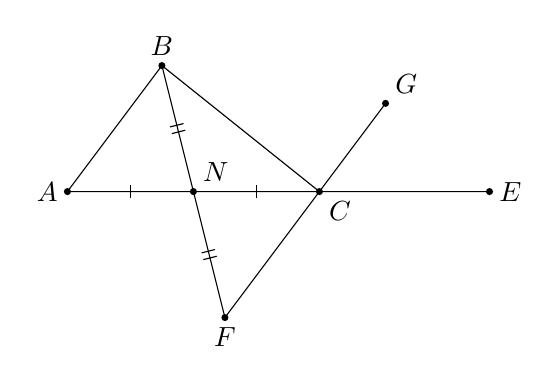
\begin{tikzpicture}[scale=.8]
\coordinate (A) at (-2,0);\coordinate (B) at (-.5,2);\coordinate (C) at (2,0);\coordinate (E) at (4.7,0);\coordinate (N) at (0,0);\coordinate (F) at (.5,-2);\coordinate (G) at (3.05,1.4);
\draw (A)--(E) (A)--(B)--(C) (B)--(F)--(G);
\path (A)--(N) node[midway,sloped,inner sep=0pt] {\krastineszymek{0}}
      (N)--(C) node[midway,sloped,inner sep=0pt] {\krastineszymek{0}}
      (B)--(N) node[midway,sloped,inner sep=0pt] {\krastineszymek{-1.25,1.25}}
      (N)--(F) node[midway,sloped,inner sep=0pt] {\krastineszymek{-1.25,1.25}};
\foreach \p/\pos in {A/left,B/above,C/below right,E/right,N/above right,F/below,G/above right}
{\fill (\p) circle (1.6pt) node[\pos] {$\p$};}
\end{tikzpicture}
\end{center}
\item Įrodykite, kad spindulys $CG$ eina kampo $BCE$ viduje, ir išveskite, kad $\angle BCE>\angle BAC$.
\item Remdamiesi b) ir d) dalių išvadomis, įrodykite, kad priekampis $BCE$ yra didesnis už kiekvieną jam negretutinį trikampio $ABC$ kampą.
\end{enumerate}
\end{staranchorproblem}
\begin{problem}\label{uzd:priekampis-pratimai} Trikampio $ABC$ priekampis prie $C$ lygus $100^\circ$. Ar kampas $A$ gali būti lygus $100^\circ$? Ar jis gali būti didesnis negu $100^\circ$? Pagrįskite. \end{problem}
\begin{problem}\label{uzd:priekampis-taikymas} Trikampio vienas kampas lygus $110^\circ$. Naudodamiesi tik priekampio nelygybe įrodykite, kad kiti du kampai yra smailieji. \end{problem}
\begin{problem}\label{uzd:priekampis-suma} Įrodykite, kad bet kurių dviejų trikampio kampų suma mažesnė už $180^\circ$. Išveskite, kad trikampyje gali būti ne daugiau kaip vienas statusis arba bukasis kampas. \end{problem}
\begin{anchorproblem}[Statmens vienatinumas]\label{atr:statmuo} Iki šiol be įrodymo rėmėmės tuo, kad per tašką, nepriklausantį tiesei, galima nubrėžti tik vieną tai tiesei statmeną tiesę. Įrodykite tai. \end{anchorproblem}
\begin{starproblem}\label{uzd:priekampis-pusiaukrastine} Trikampio $ABC$ pusiaukraštinė $AM$ yra ir kampo $BAC$ pusiaukampinė. Įrodykite, kad $AB=AC$.
\par\emph{Nurodymas.} Pratęskite pusiaukraštinę dvigubai, kaip \ref{atr:priekampis-nelygybe} uždavinio a) dalyje, ir ieškokite lygiašonio trikampio. \end{starproblem}

\section{Atkarpos vidurio statmuo}
\kelias{Kur einame.} Kur yra visi taškai, vienodai nutolę nuo dviejų duotų taškų? Atsakymą sudaro du teiginiai – savybė ir jai atvirkštinis teiginys (požymis), – ir abu įrodomi jau žinomais požymiais. Atkreipkite dėmesį, kaip skiriasi šie teiginiai ir kodėl taškus, esančius pačioje atkarpos tiesėje, tenka nagrinėti atskirai.
\Needspace{10\baselineskip}
\begin{definition}\label{apib:vidurio-statmuo} Atkarpos \emph{vidurio statmuo} yra tiesė, einanti per atkarpos vidurio tašką ir statmena tai atkarpai.
\begin{center}
\begin{tikzpicture}[scale=.8]
\coordinate (A) at (-1.5,0);\coordinate (B) at (1.5,0);\coordinate (M) at (0,0);
\draw (A)--(B) (0,-1)--(0,1.4) node[above] {$m$};
\draw (.25,0)--(.25,.25)--(0,.25);
\path (A)--(M) node[midway,sloped,inner sep=0pt] {\krastineszymek{0}}
      (M)--(B) node[midway,sloped,inner sep=0pt] {\krastineszymek{0}};
\foreach \p/\pos in {A/left,B/right,M/below left} {\fill (\p) circle (1.6pt) node[\pos] {$\p$};}
\end{tikzpicture}
\end{center}
\end{definition}
\begin{problem}\label{uzd:vidurio-supratimas-01} Atkarpos $AB$ vidurio taškas yra $M$. Tiesė $m$ eina per $M$. Kokios dar sąlygos reikia, kad $m$ būtų $AB$ vidurio statmuo? Ar tiesė, kuri statmena $AB$ taške $A$, yra $AB$ vidurio statmuo? \end{problem}
\begin{anchorproblem}[Atkarpos vidurio statmens savybė]\label{atr:vidurio-savybe} Įrodykite, jog kiekvienas atkarpos vidurio statmens taškas yra vienodai nutolęs nuo jos galų. \end{anchorproblem}
\begin{problem}\label{uzd:vidurio-savybe-01} Taškas $P$ yra atkarpos $AB$ vidurio statmenyje, $PA=8$ cm. Raskite $PB$. \end{problem}
\begin{problem}\label{uzd:vidurio-savybe-02} Atkarpos $AB$ vidurio statmuo eina per taškus $P$ ir $Q$. Įrodykite, kad $\angle APQ=\angle QPB$, jei $P\ne Q$ ir $P$ nėra tiesėje $AB$. \end{problem}
\begin{anchorproblem}[Vidurio statmens požymis]\label{atr:vidurio-atvirkstine} Įrodykite: jei taškas vienodai nutolęs nuo atkarpos galų, tai jis yra tos atkarpos vidurio statmenyje. Atskirai aptarkite atvejį, kai taškas yra pačioje tiesėje, kuriai priklauso atkarpa. \end{anchorproblem}
\begin{problem}\label{uzd:vidurio-atvirkstine-01} Žinoma, kad $XA=XB$ ir $YA=YB$, o $X\ne Y$. Įrodykite, kad tiesė $XY$ yra atkarpos $AB$ vidurio statmuo. \end{problem}
\begin{problem}\label{uzd:vidurio-taikymas-01} Atkarpos $AB$ vidurio statmenyje yra taškas $P$, nepriklausantis tiesei $AB$. Taškas $M$ yra atkarpos $AB$ vidurys, $AB=10$ cm, o trikampio $PAB$ perimetras lygus $24$ cm. Raskite $PA$, $PB$ ir $AM$. \end{problem}
\begin{problem}\label{uzd:vidurio-taikymas-02} Trikampio $ABC$ pusiaukraštinė $AM$ yra ir aukštinė. Įrodykite, kad $AB=AC$. \end{problem}
\begin{starproblem}\label{uzd:vidurio-taikymas-03} Trikampyje $ABC$ duota $AB=AC$, $M$ yra kraštinės $BC$ vidurio taškas. Kraštinių $AB$ ir $AC$ vidurio statmenys kertasi taške $O$. Įrodykite, kad $OB=OC$ ir kad taškas $O$ priklauso tiesei $AM$. \end{starproblem}
\section*{Svarbiausios temos išvados}
Prieš skaitydami pabandykite atsakyti: kaip parenkamos atitinkamos viršūnės? Kaip iš trikampių lygumo gaunama atkarpų lygybė? Kuo skiriasi savybė nuo jai atvirkštinio teiginio?
\begin{itemize}
\item Trikampiams palyginti taikome tris požymius: dvi kraštines ir kampą tarp jų; kraštinę ir du kampus prie jos; tris kraštines (\ref{atr:sss-poz}). Atitinkamas viršūnes rašome ta pačia tvarka.
\item Lygios dvi kraštinės ir bet kuris kampas savaime nesudaro pirmojo požymio: kampas turi būti tarp tų kraštinių (\ref{uzd:lygybe-ssa-01}).
\item Lygiašonio trikampio pagrindo kampai lygūs (\ref{atr:lygias-pagrindo-kampai}); jei du trikampio kampai lygūs, tai trikampis lygiašonis (\ref{atr:lygias-atvirkstine}).
\item Lygiašonio trikampio pusiaukraštinė į pagrindą yra ir aukštinė, ir pusiaukampinė (\ref{atr:lygias-pusiaukrastine}). Atvirkščiai: jei pusiaukraštinė yra pusiaukampinė (\ref{uzd:priekampis-pusiaukrastine}) arba aukštinė (\ref{uzd:vidurio-taikymas-02}), trikampis lygiašonis.
\item Trikampio priekampis didesnis už kiekvieną jam negretutinį trikampio kampą (\ref{atr:priekampis-nelygybe}). Todėl dviejų trikampio kampų suma mažesnė už $180^\circ$ (\ref{uzd:priekampis-suma}), o per tašką, nepriklausantį tiesei, eina vienintelis jai statmuo (\ref{atr:statmuo}).
\item Atkarpos vidurio statmens taškai ir tik jie vienodai nutolę nuo jos galų (\ref{atr:vidurio-savybe}, \ref{atr:vidurio-atvirkstine}).
\end{itemize}
\textbf{Metodai, kuriuos išmokome.} Papildoma linija, sukurianti lygius trikampius (pusiaukampinė lygiašoniame trikampyje). Trikampio palyginimas su juo pačiu. Du lygiašoniai trikampiai su bendru pagrindu. Pusiaukraštinės pratęsimas dvigubai. Atvejų nagrinėjimas pagal taškų išsidėstymą: brėžinys rodo tik vieną atvejį.
\section*{Atraminiai faktai: vaizdinė santrauka}
Vienodi brūkšneliai žymi lygias atkarpas, o vienodos graikiškos raidės – lygius kampus. Nuorodos nurodo atitinkamus atraminius uždavinius.

\Needspace{13\baselineskip}
\textbf{Lygiašonio trikampio savybė ir požymis} (\ref{atr:lygias-pagrindo-kampai}, \ref{atr:lygias-atvirkstine})
\begin{center}
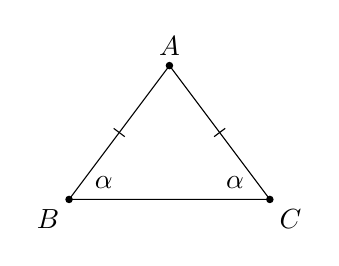
\begin{tikzpicture}[scale=.85]
\coordinate (A) at (1.5,2); \coordinate (B) at (0,0); \coordinate (C) at (3,0);
\draw (A)--(B) node[midway,sloped,inner sep=0pt] {\krastineszymek{0}}
      --(C)--(A) node[midway,sloped,inner sep=0pt] {\krastineszymek{0}};
\node at (.52,.25) {$\alpha$}; \node at (2.48,.25) {$\alpha$};
\foreach \p/\pos in {A/above,B/below left,C/below right} {\fill (\p) circle (1.6pt) node[\pos] {$\p$};}
\end{tikzpicture}
\end{center}
Jei $AB=AC$, tai $\angle ABC=\angle BCA$. Ir atvirkščiai: jei $\angle ABC=\angle BCA$, tai $AB=AC$.

\Needspace{14\baselineskip}
\textbf{Pusiaukraštinė į lygiašonio trikampio pagrindą} (\ref{atr:lygias-pusiaukrastine})
\begin{center}
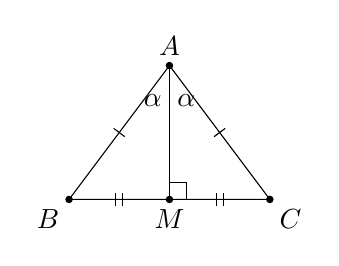
\begin{tikzpicture}[scale=.85]
\coordinate (A) at (1.5,2); \coordinate (B) at (0,0); \coordinate (C) at (3,0); \coordinate (M) at (1.5,0);
\draw (A)--(B) node[midway,sloped,inner sep=0pt] {\krastineszymek{0}}
      --(C)--(A) node[midway,sloped,inner sep=0pt] {\krastineszymek{0}};
\draw (A)--(M);
\path (B)--(M) node[midway,sloped,inner sep=0pt] {\krastineszymek{-1.25,1.25}}
      (M)--(C) node[midway,sloped,inner sep=0pt] {\krastineszymek{-1.25,1.25}};
\draw (1.5,.25)--(1.75,.25)--(1.75,0);
\node at (1.25,1.48) {$\alpha$}; \node at (1.75,1.48) {$\alpha$};
\foreach \p/\pos in {A/above,B/below left,C/below right,M/below} {\fill (\p) circle (1.6pt) node[\pos] {$\p$};}
\end{tikzpicture}
\end{center}
Jei $AB=AC$ ir $BM=MC$, tai pusiaukraštinė $AM$ yra ir aukštinė, ir kampo $BAC$ pusiaukampinė: $AM\perp BC$, $\angle BAM=\angle MAC$.

\Needspace{13\baselineskip}
\textbf{Lygiakraščio trikampio savybė ir požymis} (\ref{atr:lygiakrastis-kampai})
\begin{center}
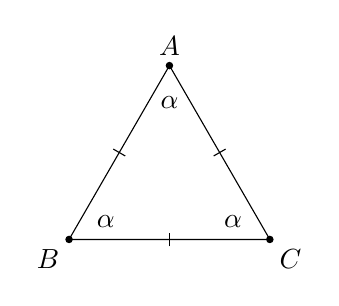
\begin{tikzpicture}[scale=.85]
\coordinate (A) at (1.5,2.598); \coordinate (B) at (0,0); \coordinate (C) at (3,0);
\draw (A)--(B) node[midway,sloped,inner sep=0pt] {\krastineszymek{0}}
      --(C) node[midway,sloped,inner sep=0pt] {\krastineszymek{0}}
      --(A) node[midway,sloped,inner sep=0pt] {\krastineszymek{0}};
\node at (1.5,2.05) {$\alpha$}; \node at (.55,.27) {$\alpha$}; \node at (2.45,.27) {$\alpha$};
\foreach \p/\pos in {A/above,B/below left,C/below right} {\fill (\p) circle (1.6pt) node[\pos] {$\p$};}
\end{tikzpicture}
\end{center}
Trikampis yra lygiakraštis tada ir tik tada, kai visi jo kampai lygūs.

\Needspace{14\baselineskip}
\textbf{Trikampių lygumo požymis pagal tris kraštines} (\ref{atr:sss-poz})
\begin{center}
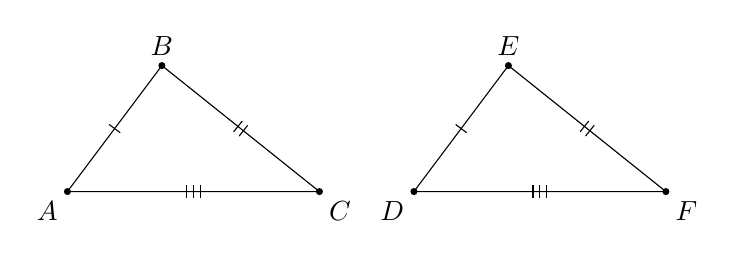
\begin{tikzpicture}[scale=.8]
\coordinate (A) at (0,0); \coordinate (B) at (1.5,2); \coordinate (C) at (4,0);
\coordinate (D) at (5.5,0); \coordinate (E) at (7,2); \coordinate (F) at (9.5,0);
\draw (A)--(B) node[midway,sloped,inner sep=0pt] {\krastineszymek{0}}
      --(C) node[midway,sloped,inner sep=0pt] {\krastineszymek{-1.25,1.25}}
      --(A) node[midway,sloped,inner sep=0pt] {\krastineszymek{-2.5,0,2.5}};
\draw (D)--(E) node[midway,sloped,inner sep=0pt] {\krastineszymek{0}}
      --(F) node[midway,sloped,inner sep=0pt] {\krastineszymek{-1.25,1.25}}
      --(D) node[midway,sloped,inner sep=0pt] {\krastineszymek{-2.5,0,2.5}};
\foreach \p/\pos in {A/below left,B/above,C/below right,D/below left,E/above,F/below right} {\fill (\p) circle (1.6pt) node[\pos] {$\p$};}
\end{tikzpicture}
\end{center}
Jei $AB=DE$, $BC=EF$ ir $AC=DF$, tai $\triangle ABC=\triangle DEF$. Atitinkamos viršūnės rašomos ta pačia tvarka.

\Needspace{13\baselineskip}
\textbf{Trikampio priekampio nelygybė} (\ref{atr:priekampis-nelygybe})
\begin{center}
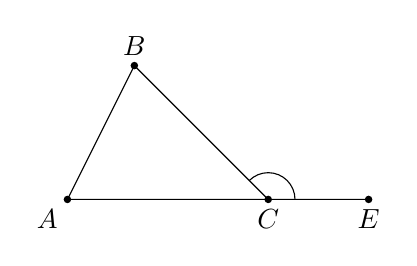
\begin{tikzpicture}[scale=.85]
\coordinate (A) at (0,0); \coordinate (B) at (1,2); \coordinate (C) at (3,0); \coordinate (E) at (4.5,0);
\draw (A)--(B)--(C)--(E) (A)--(C);
\draw (3.4,0) arc[start angle=0,end angle=135,radius=.4];
\foreach \p/\pos in {A/below left,B/above,C/below,E/below} {\fill (\p) circle (1.6pt) node[\pos] {$\p$};}
\end{tikzpicture}
\end{center}
Priekampis $\angle BCE$ yra didesnis už kiekvieną jam negretutinį trikampio kampą:
$\angle BCE>\angle BAC$ ir $\angle BCE>\angle ABC$.

\Needspace{14\baselineskip}
\textbf{Atkarpos vidurio statmens savybė ir požymis} (\ref{atr:vidurio-savybe}, \ref{atr:vidurio-atvirkstine})
\begin{center}
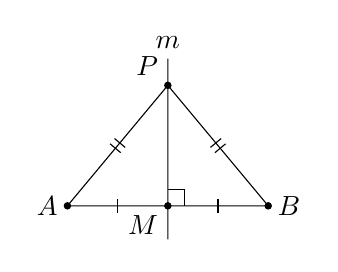
\begin{tikzpicture}[scale=.85]
\coordinate (A) at (0,0); \coordinate (B) at (3,0); \coordinate (M) at (1.5,0); \coordinate (P) at (1.5,1.8);
\draw (A)--(B) (1.5,-.5)--(1.5,2.2) node[above] {$m$} (A)--(P)--(B);
\draw (1.5,.25)--(1.75,.25)--(1.75,0);
\path (A)--(M) node[midway,sloped,inner sep=0pt] {\krastineszymek{0}}
      (M)--(B) node[midway,sloped,inner sep=0pt] {\krastineszymek{0}}
      (A)--(P) node[midway,sloped,inner sep=0pt] {\krastineszymek{-1.25,1.25}}
      (B)--(P) node[midway,sloped,inner sep=0pt] {\krastineszymek{-1.25,1.25}};
\foreach \p/\pos in {A/left,B/right,M/below left,P/above left} {\fill (\p) circle (1.6pt) node[\pos] {$\p$};}
\end{tikzpicture}
\end{center}
Jei $m$ yra $AB$ vidurio statmuo, tai kiekvienam $P\in m$ galioja $PA=PB$. Ir atvirkščiai: jei $PA=PB$, tai $P\in m$. Tai galioja ir tada, kai $P=M$.

\section*{Savikontrolė}
\setcounter{theorem}{0}\renewcommand{\thetheorem}{S\arabic{theorem}}\renewcommand{\theHtheorem}{S\arabic{theorem}}
Spręskite nežiūrėdami į ankstesnius skyrius.
\begin{problem}\label{uzd:savikontrole-01} Atkarpos $AD$ ir $BC$ kertasi taške $O$, $AO=OD$, $BO=OC$. Įrodykite, kad $AC=DB$ ir $\angle ACB=\angle DBC$. \end{problem}
\begin{problem}\label{uzd:savikontrole-02} Trikampyje $XYZ$ žinoma $XY=XZ$, $\angle XYZ=4t+3^\circ$, $\angle YZX=5t-9^\circ$. Raskite $t$ ir šiuos kampus. \end{problem}
\begin{problem}\label{uzd:savikontrole-03} Taškas $M$ yra atkarpos $AB$ vidurys, o taškas $P$ tenkina lygybę $PA=PB$. Ar teisinga, kad tiesė $PM$ yra atkarpos $AB$ vidurio statmuo? Paaiškinkite. \end{problem}
\begin{problem}\label{uzd:savikontrole-04} Trikampyje $ABC$ duota $\angle ABC=\angle ACB$, o taškai $D$ ir $E$ yra kraštinėje $BC$, $BD=CE$. Įrodykite, kad $AD=AE$. \end{problem}
\begin{problem}\label{uzd:savikontrole-05} Trikampio $ABC$ aukštinė $AH$ yra ir kampo $BAC$ pusiaukampinė. Įrodykite, kad $AB=AC$ ir $BH=HC$. \end{problem}
\begin{problem}\label{uzd:savikontrole-06} Lygiakraščio trikampio $ABC$ kraštinių $AB$, $BC$, $CA$ vidiniuose taškuose $K$, $L$, $M$ pažymėti taip, kad $AK=BL=CM$. Įrodykite, kad trikampis $KLM$ lygiakraštis. \end{problem}
\begin{problem}\label{uzd:savikontrole-07} Trikampiuose $ABC$ ir $PQR$ duota $AB=QR$, $BC=RP$ ir $AC=QP$. Ar trikampiai lygūs? Jei taip, užrašykite jų lygybę tinkama viršūnių tvarka ir nurodykite kampą, atitinkantį $\angle ABC$. \end{problem}
\begin{problem}\label{uzd:savikontrole-08} Trikampio $ABC$ kraštinė $AC$ pratęsta už $C$ iki taško $E$. Žinoma, kad $\angle BCE=110^\circ$. Kokias nelygybes galima užrašyti palyginus šį priekampį su kampais $BAC$ ir $ABC$? Pagrįskite. \end{problem}
\begin{problem}\label{uzd:savikontrole-09} Taškas $M$ yra atkarpos $AB$ vidurys, o tiesė $m$ yra šios atkarpos vidurio statmuo. Taškas $P$ priklauso tiesei $m$, o taškas $Q$ tenkina lygybę $QA=QB$. Ką galima pasakyti apie $PA$ ir $PB$? Ar $Q$ būtinai priklauso tiesei $m$? Ar išvada apie $Q$ galioja, jei $Q$ yra tiesėje $AB$? Pagrįskite. \end{problem}
\begin{problem}\label{uzd:savikontrole-10} Taškas $P$, skirtingas nuo $A$, yra kampo $XAY$ pusiaukampinėje, o taškai $B$ ir $C$ – atitinkamai kampo kraštinėse $AX$ ir $AY$, be to, $AB=AC$. Įrodykite, kad $PB=PC$. \end{problem}
\begin{problem}\label{uzd:savikontrole-11} Trikampyje $ABC$ duota $AB=AC$. Taškas $D$ yra kraštinės $AB$, o taškas $E$ – kraštinės $AC$ vidinis taškas, $AD=AE$. Įrodykite, kad $BE=CD$. \end{problem}
\begin{problem}\label{uzd:savikontrole-12} Lygiašonio trikampio perimetras yra $30$ cm, o viena kraštinė lygi $7$ cm. Raskite likusias dvi kraštines. \end{problem}
\section*{Atsakymai}
\textbf{\ref{uzd:lygybe-atitikimas-01}.} $PQ$, $PR$; $\angle PQR$, $\angle QPR$; $BC=QR$, $\angle ACB=\angle PRQ$.\par
\textbf{\ref{uzd:lygybe-sas-01}.} $BC=ED$.\par
\textbf{\ref{uzd:lygybe-asa-01}.} $AC=KM$.\par
\textbf{\ref{uzd:lygybe-ssa-01}.} Ne.\par
\textbf{\ref{uzd:lygias-perimetras-01}.} $7$ cm ir $7$ cm arba $6$ cm ir $8$ cm.\par
\textbf{\ref{uzd:lygias-kampai-01}.} $38^\circ$; ne.\par
\textbf{\ref{uzd:lygias-kampai-02}.} $x=15$, abu kampai po $40^\circ$.\par
\textbf{\ref{uzd:lygias-atvirkstine-01}.} $7$ cm.\par
\textbf{\ref{uzd:lygias-atvirkstine-02}.} $KM=LM$.\par
\textbf{\ref{uzd:lygias-pusiaukrastine-01}.} $27^\circ$ ir $90^\circ$.\par
\textbf{\ref{uzd:sss-tiesioginis-01}.} $\triangle ABC=\triangle PRQ$.\par
\textbf{\ref{uzd:sss-konstr-01}.} Vienas.\par
\textbf{\ref{uzd:priekampis-pratimai}.} Ne; ne.\par
\textbf{\ref{uzd:vidurio-savybe-01}.} $8$ cm.\par
\textbf{\ref{uzd:vidurio-taikymas-01}.} $PA=PB=7$ cm, $AM=5$ cm.\par
\textbf{\ref{uzd:savikontrole-02}.} $t=12$, abu kampai po $51^\circ$.\par
\textbf{\ref{uzd:savikontrole-03}.} Taip, jei $P\ne M$; kai $P=M$, tiesė $PM$ neapibrėžta.\par
\textbf{\ref{uzd:savikontrole-07}.} Taip, $\triangle ABC=\triangle QRP$; $\angle QRP$.\par
\textbf{\ref{uzd:savikontrole-08}.} $\angle BAC<110^\circ$, $\angle ABC<110^\circ$.\par
\textbf{\ref{uzd:savikontrole-09}.} $PA=PB$; taip; taip.\par
\textbf{\ref{uzd:savikontrole-12}.} $11{,}5$ cm ir $11{,}5$ cm.\par

\section*{Sprendimai ir įrodymai}
Šiame skyriuje įrodymai pateikiami kaupiamuoju principu: kiekvienam naujam sąlygos faktui ar įrodymo žingsniui pateikiamas atskiras brėžinys, kuriame naujai pridėtas arba išryškintas elementas pažymėtas \textcolor{blue}{mėlynai}, o ankstesnių žingsnių duomenys išlieka juodi.

\begin{solution}[\ref{uzd:breziniai-lygumas-01}]
\textbf{(1)}
\par\emph{1 žingsnis.} Duota $AO=CO$ (pažymime vienu brūkšneliu):
\begin{center}
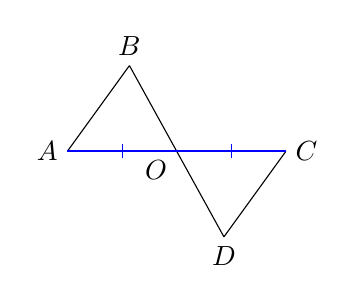
\begin{tikzpicture}[scale=0.75]
\coordinate (A) at (-1.85,0); \coordinate (O) at (0,0); \coordinate (C) at (1.85,0);
\coordinate (B) at (-0.8,1.45); \coordinate (D) at (0.8,-1.45);
\draw (A)--(C) (B)--(D) (A)--(B) (C)--(D);
\draw[blue,thick] (A)--(O) node[midway,sloped,inner sep=0pt] {\krastineszymek{0}} (O)--(C) node[midway,sloped,inner sep=0pt] {\krastineszymek{0}};
\node[left] at (A) {$A$}; \node[right] at (C) {$C$}; \node[above] at (B) {$B$}; \node[below] at (D) {$D$}; \node[below left] at (O) {$O$};
\end{tikzpicture}
\end{center}
\par\emph{2 žingsnis.} Duota $\angle BAO=\angle DCO$ (pridedame po vieną lankelį):
\begin{center}
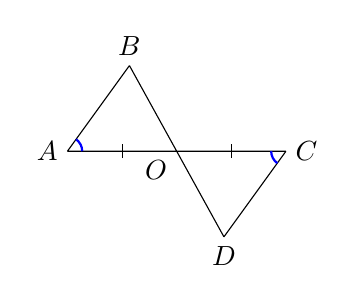
\begin{tikzpicture}[scale=0.75]
\coordinate (A) at (-1.85,0); \coordinate (O) at (0,0); \coordinate (C) at (1.85,0);
\coordinate (B) at (-0.8,1.45); \coordinate (D) at (0.8,-1.45);
\draw (A)--(C) (B)--(D) (A)--(B) (C)--(D);
\path (A)--(O) node[midway,sloped,inner sep=0pt] {\krastineszymek{0}} (O)--(C) node[midway,sloped,inner sep=0pt] {\krastineszymek{0}};
\draw[blue,thick] (-1.7034,0.2025) arc[start angle=54.09,end angle=0,radius=0.25];
\draw[blue,thick] (1.7034,-0.2025) arc[start angle=-125.91,end angle=-180,radius=0.25];
\node[left] at (A) {$A$}; \node[right] at (C) {$C$}; \node[above] at (B) {$B$}; \node[below] at (D) {$D$}; \node[below left] at (O) {$O$};
\end{tikzpicture}
\end{center}
\par\emph{3 žingsnis.} Kryžminiai kampai $\angle AOB$ ir $\angle COD$ lygūs (pridedame dvigubus lankelius). Kadangi lygūs kampai yra prie atitinkamai lygių kraštinių $AO$ ir $CO$, gauname $\triangle AOB=\triangle COD$ pagal kraštinę ir du kampus prie jos:
\begin{center}
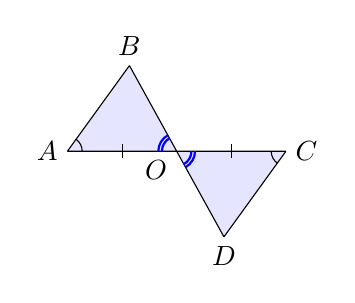
\begin{tikzpicture}[scale=0.75]
\coordinate (A) at (-1.85,0); \coordinate (O) at (0,0); \coordinate (C) at (1.85,0);
\coordinate (B) at (-0.8,1.45); \coordinate (D) at (0.8,-1.45);
\fill[blue!10] (A)--(O)--(B)--cycle (C)--(O)--(D)--cycle;
\draw (A)--(C) (B)--(D) (A)--(B) (C)--(D);
\path (A)--(O) node[midway,sloped,inner sep=0pt] {\krastineszymek{0}} (O)--(C) node[midway,sloped,inner sep=0pt] {\krastineszymek{0}};
\draw (-1.7034,0.2025) arc[start angle=54.09,end angle=0,radius=0.25];
\draw (1.7034,-0.2025) arc[start angle=-125.91,end angle=-180,radius=0.25];
\draw[blue,thick] (-0.12,0.22) arc[start angle=118.8,end angle=180,radius=0.25];
\draw[blue,thick] (-0.15,0.27) arc[start angle=118.8,end angle=180,radius=0.31];
\draw[blue,thick] (0.12,-0.22) arc[start angle=-61.2,end angle=0,radius=0.25];
\draw[blue,thick] (0.15,-0.27) arc[start angle=-61.2,end angle=0,radius=0.31];
\node[left] at (A) {$A$}; \node[right] at (C) {$C$}; \node[above] at (B) {$B$}; \node[below] at (D) {$D$}; \node[below left] at (O) {$O$};
\end{tikzpicture}
\end{center}

\textbf{(2)}
\par\emph{1 žingsnis.} Duota $AO=CO$ (vienas brūkšnelis):
\begin{center}
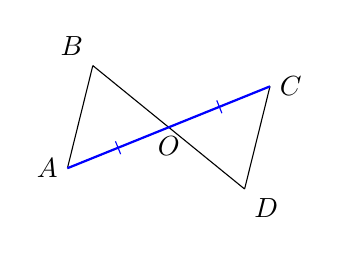
\begin{tikzpicture}[scale=0.75]
\coordinate (A) at (-1.715,-0.693); \coordinate (O) at (0,0); \coordinate (C) at (1.715,0.693);
\coordinate (B) at (-1.285,1.045); \coordinate (D) at (1.285,-1.045);
\draw (A)--(C) (B)--(D) (A)--(B) (C)--(D);
\draw[blue,thick] (A)--(O) node[midway,sloped,inner sep=0pt] {\krastineszymek{0}} (O)--(C) node[midway,sloped,inner sep=0pt] {\krastineszymek{0}};
\node[left] at (A) {$A$}; \node[right] at (C) {$C$}; \node[above left] at (B) {$B$}; \node[below right] at (D) {$D$}; \node[below] at (O) {$O$};
\end{tikzpicture}
\end{center}
\par\emph{2 žingsnis.} Duota $BO=DO$ (pridedame po du brūkšnelius):
\begin{center}
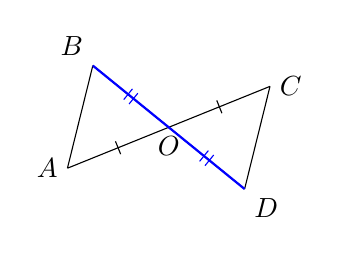
\begin{tikzpicture}[scale=0.75]
\coordinate (A) at (-1.715,-0.693); \coordinate (O) at (0,0); \coordinate (C) at (1.715,0.693);
\coordinate (B) at (-1.285,1.045); \coordinate (D) at (1.285,-1.045);
\draw (A)--(C) (B)--(D) (A)--(B) (C)--(D);
\path (A)--(O) node[midway,sloped,inner sep=0pt] {\krastineszymek{0}} (O)--(C) node[midway,sloped,inner sep=0pt] {\krastineszymek{0}};
\draw[blue,thick] (B)--(O) node[midway,sloped,inner sep=0pt] {\krastineszymek{-1.25,1.25}} (O)--(D) node[midway,sloped,inner sep=0pt] {\krastineszymek{-1.25,1.25}};
\node[left] at (A) {$A$}; \node[right] at (C) {$C$}; \node[above left] at (B) {$B$}; \node[below right] at (D) {$D$}; \node[below] at (O) {$O$};
\end{tikzpicture}
\end{center}
\par\emph{3 žingsnis.} Kryžminiai kampai $\angle AOB$ ir $\angle COD$ lygūs (pridedame lankelius tarp lygių kraštinių). Todėl $\triangle AOB=\triangle COD$ pagal dvi kraštines ir kampą tarp jų:
\begin{center}
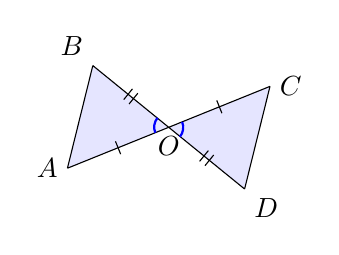
\begin{tikzpicture}[scale=0.75]
\coordinate (A) at (-1.715,-0.693); \coordinate (O) at (0,0); \coordinate (C) at (1.715,0.693);
\coordinate (B) at (-1.285,1.045); \coordinate (D) at (1.285,-1.045);
\fill[blue!10] (A)--(O)--(B)--cycle (C)--(O)--(D)--cycle;
\draw (A)--(C) (B)--(D) (A)--(B) (C)--(D);
\path (A)--(O) node[midway,sloped,inner sep=0pt] {\krastineszymek{0}} (O)--(C) node[midway,sloped,inner sep=0pt] {\krastineszymek{0}}
      (B)--(O) node[midway,sloped,inner sep=0pt] {\krastineszymek{-1.25,1.25}} (O)--(D) node[midway,sloped,inner sep=0pt] {\krastineszymek{-1.25,1.25}};
\draw[blue,thick] (-0.19,0.16) arc[start angle=140.9,end angle=202,radius=0.25];
\draw[blue,thick] (0.19,-0.16) arc[start angle=-39.1,end angle=22,radius=0.25];
\node[left] at (A) {$A$}; \node[right] at (C) {$C$}; \node[above left] at (B) {$B$}; \node[below right] at (D) {$D$}; \node[below] at (O) {$O$};
\end{tikzpicture}
\end{center}

\textbf{(3)}
\par\emph{1 žingsnis.} Duota $AC=AD$:
\begin{center}
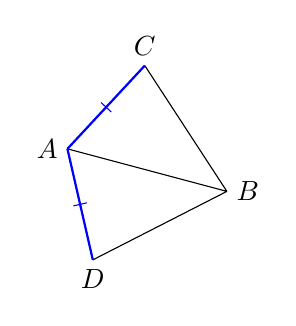
\begin{tikzpicture}[scale=0.75]
\coordinate (A) at (0,0); \coordinate (B) at (2.7,-0.72); \coordinate (C) at (1.31,1.41); \coordinate (D) at (0.43,-1.88);
\draw (A)--(B) (A)--(C) (B)--(C) (A)--(D) (B)--(D);
\draw[blue,thick] (A)--(C) node[midway,sloped,inner sep=0pt] {\krastineszymek{0}} (A)--(D) node[midway,sloped,inner sep=0pt] {\krastineszymek{0}};
\node[left] at (A) {$A$}; \node[right] at (B) {$B$}; \node[above] at (C) {$C$}; \node[below] at (D) {$D$};
\end{tikzpicture}
\end{center}
\par\emph{2 žingsnis.} Duota $\angle CAB=\angle DAB$:
\begin{center}
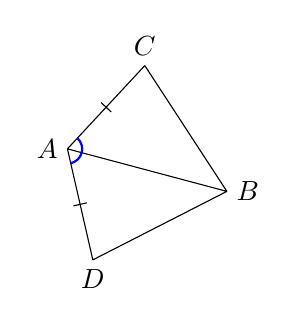
\begin{tikzpicture}[scale=0.75]
\coordinate (A) at (0,0); \coordinate (B) at (2.7,-0.72); \coordinate (C) at (1.31,1.41); \coordinate (D) at (0.43,-1.88);
\draw (A)--(B) (A)--(C) (B)--(C) (A)--(D) (B)--(D);
\path (A)--(C) node[midway,sloped,inner sep=0pt] {\krastineszymek{0}} (A)--(D) node[midway,sloped,inner sep=0pt] {\krastineszymek{0}};
\draw[blue,thick] (0.17,0.18) arc[start angle=47.1,end angle=-15,radius=0.25];
\draw[blue,thick] (0.056,-0.244) arc[start angle=-77.1,end angle=-15,radius=0.25];
\node[left] at (A) {$A$}; \node[right] at (B) {$B$}; \node[above] at (C) {$C$}; \node[below] at (D) {$D$};
\end{tikzpicture}
\end{center}
\par\emph{3 žingsnis.} Kraštinė $AB$ yra bendra (pažymime dviem brūkšneliais). Todėl $\triangle CAB=\triangle DAB$ pagal dvi kraštines ir kampą tarp jų:
\begin{center}
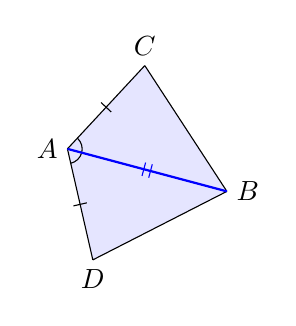
\begin{tikzpicture}[scale=0.75]
\coordinate (A) at (0,0); \coordinate (B) at (2.7,-0.72); \coordinate (C) at (1.31,1.41); \coordinate (D) at (0.43,-1.88);
\fill[blue!10] (A)--(B)--(C)--cycle (A)--(B)--(D)--cycle;
\draw (A)--(B) (A)--(C) (B)--(C) (A)--(D) (B)--(D);
\path (A)--(C) node[midway,sloped,inner sep=0pt] {\krastineszymek{0}} (A)--(D) node[midway,sloped,inner sep=0pt] {\krastineszymek{0}};
\draw (0.17,0.18) arc[start angle=47.1,end angle=-15,radius=0.25];
\draw (0.056,-0.244) arc[start angle=-77.1,end angle=-15,radius=0.25];
\draw[blue,thick] (A)--(B) node[midway,sloped,inner sep=0pt] {\krastineszymek{-1.25,1.25}};
\node[left] at (A) {$A$}; \node[right] at (B) {$B$}; \node[above] at (C) {$C$}; \node[below] at (D) {$D$};
\end{tikzpicture}
\end{center}

\textbf{(4)}
\par\emph{1 žingsnis.} Duota $\angle CAB=\angle DAB$:
\begin{center}
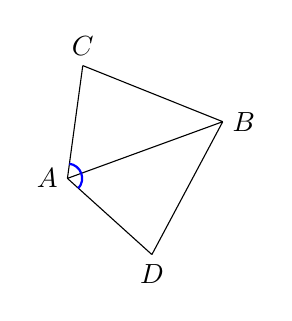
\begin{tikzpicture}[scale=0.75]
\coordinate (A) at (0,0); \coordinate (B) at (2.63,0.96); \coordinate (C) at (0.26,1.91); \coordinate (D) at (1.43,-1.29);
\draw (A)--(B) (A)--(C) (B)--(C) (A)--(D) (B)--(D);
\draw[blue,thick] (0.034,0.248) arc[start angle=82.1,end angle=20,radius=0.25];
\draw[blue,thick] (0.185,-0.168) arc[start angle=-42.1,end angle=20,radius=0.25];
\node[left] at (A) {$A$}; \node[right] at (B) {$B$}; \node[above] at (C) {$C$}; \node[below] at (D) {$D$};
\end{tikzpicture}
\end{center}
\par\emph{2 žingsnis.} Duota $\angle ABC=\angle ABD$:
\begin{center}
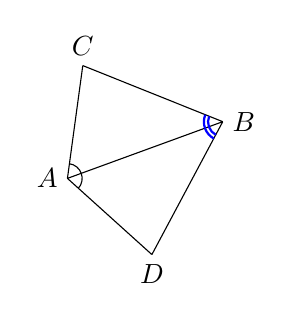
\begin{tikzpicture}[scale=0.75]
\coordinate (A) at (0,0); \coordinate (B) at (2.63,0.96); \coordinate (C) at (0.26,1.91); \coordinate (D) at (1.43,-1.29);
\draw (A)--(B) (A)--(C) (B)--(C) (A)--(D) (B)--(D);
\draw (0.034,0.248) arc[start angle=82.1,end angle=20,radius=0.25];
\draw (0.185,-0.168) arc[start angle=-42.1,end angle=20,radius=0.25];
\draw[blue,thick] (2.396,0.872) arc[start angle=-160,end angle=-201.8,radius=0.25];
\draw[blue,thick] (2.33,0.848) arc[start angle=-160,end angle=-201.8,radius=0.32];
\draw[blue,thick] (2.396,0.872) arc[start angle=-160,end angle=-118.2,radius=0.25];
\draw[blue,thick] (2.33,0.848) arc[start angle=-160,end angle=-118.2,radius=0.32];
\node[left] at (A) {$A$}; \node[right] at (B) {$B$}; \node[above] at (C) {$C$}; \node[below] at (D) {$D$};
\end{tikzpicture}
\end{center}
\par\emph{3 žingsnis.} Kraštinė $AB$ yra bendra, o lygūs kampai yra prie jos. Todėl $\triangle CAB=\triangle DAB$ pagal kraštinę ir du kampus prie jos:
\begin{center}
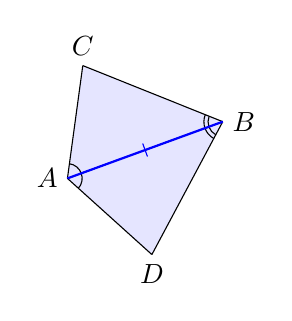
\begin{tikzpicture}[scale=0.75]
\coordinate (A) at (0,0); \coordinate (B) at (2.63,0.96); \coordinate (C) at (0.26,1.91); \coordinate (D) at (1.43,-1.29);
\fill[blue!10] (A)--(B)--(C)--cycle (A)--(B)--(D)--cycle;
\draw (A)--(B) (A)--(C) (B)--(C) (A)--(D) (B)--(D);
\draw (0.034,0.248) arc[start angle=82.1,end angle=20,radius=0.25];
\draw (0.185,-0.168) arc[start angle=-42.1,end angle=20,radius=0.25];
\draw (2.396,0.872) arc[start angle=-160,end angle=-201.8,radius=0.25];
\draw (2.33,0.848) arc[start angle=-160,end angle=-201.8,radius=0.32];
\draw (2.396,0.872) arc[start angle=-160,end angle=-118.2,radius=0.25];
\draw (2.33,0.848) arc[start angle=-160,end angle=-118.2,radius=0.32];
\draw[blue,thick] (A)--(B) node[midway,sloped,inner sep=0pt] {\krastineszymek{0}};
\node[left] at (A) {$A$}; \node[right] at (B) {$B$}; \node[above] at (C) {$C$}; \node[below] at (D) {$D$};
\end{tikzpicture}
\end{center}

\textbf{(5)}
\par\emph{1 žingsnis.} Duota $AB=AE$:
\begin{center}
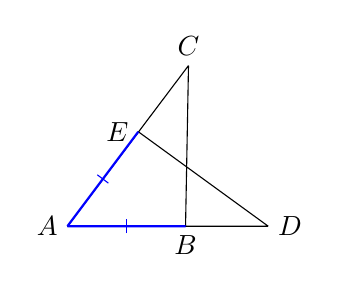
\begin{tikzpicture}[scale=0.75]
\coordinate (A) at (0,0); \coordinate (B) at (2,0); \coordinate (D) at (3.4,0);
\coordinate (C) at (2.05,2.72); \coordinate (E) at (1.2,1.6);
\draw (A)--(D) (A)--(C) (B)--(C) (D)--(E);
\draw[blue,thick] (A)--(B) node[midway,sloped,inner sep=0pt] {\krastineszymek{0}} (A)--(E) node[midway,sloped,inner sep=0pt] {\krastineszymek{0}};
\node[left] at (A) {$A$}; \node[below] at (B) {$B$}; \node[right] at (D) {$D$}; \node[above] at (C) {$C$}; \node[left] at (E) {$E$};
\end{tikzpicture}
\end{center}
\par\emph{2 žingsnis.} Duota $AC=AD$ (pažymime šias pilnas kraštines dviem brūkšneliais):
\begin{center}
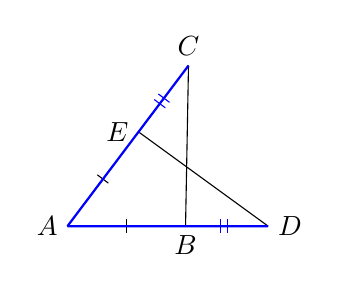
\begin{tikzpicture}[scale=0.75]
\coordinate (A) at (0,0); \coordinate (B) at (2,0); \coordinate (D) at (3.4,0);
\coordinate (C) at (2.05,2.72); \coordinate (E) at (1.2,1.6);
\draw (A)--(D) (A)--(C) (B)--(C) (D)--(E);
\path (A)--(B) node[midway,sloped,inner sep=0pt] {\krastineszymek{0}} (A)--(E) node[midway,sloped,inner sep=0pt] {\krastineszymek{0}};
\draw[blue,thick] (A)--(C) node[pos=0.78,sloped,inner sep=0pt] {\krastineszymek{-1.25,1.25}} (A)--(D) node[pos=0.78,sloped,inner sep=0pt] {\krastineszymek{-1.25,1.25}};
\node[left] at (A) {$A$}; \node[below] at (B) {$B$}; \node[right] at (D) {$D$}; \node[above] at (C) {$C$}; \node[left] at (E) {$E$};
\end{tikzpicture}
\end{center}
\par\emph{3 žingsnis.} Spindulys $AB$ sutampa su $AD$, o $AC$ – su $AE$, todėl $\angle BAC=\angle EAD$ yra bendras kampas tarp atitinkamų kraštinių. Taigi $\triangle ABC=\triangle AED$ pagal dvi kraštines ir kampą tarp jų:
\begin{center}
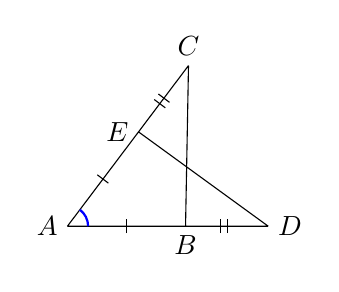
\begin{tikzpicture}[scale=0.75]
\coordinate (A) at (0,0); \coordinate (B) at (2,0); \coordinate (D) at (3.4,0);
\coordinate (C) at (2.05,2.72); \coordinate (E) at (1.2,1.6);
\draw (A)--(D) (A)--(C) (B)--(C) (D)--(E);
\path (A)--(B) node[midway,sloped,inner sep=0pt] {\krastineszymek{0}} (A)--(E) node[midway,sloped,inner sep=0pt] {\krastineszymek{0}}
      (A)--(C) node[pos=0.78,sloped,inner sep=0pt] {\krastineszymek{-1.25,1.25}} (A)--(D) node[pos=0.78,sloped,inner sep=0pt] {\krastineszymek{-1.25,1.25}};
\draw[blue,thick] (0.35,0) arc[start angle=0,end angle=53,radius=0.35];
\node[left] at (A) {$A$}; \node[below] at (B) {$B$}; \node[right] at (D) {$D$}; \node[above] at (C) {$C$}; \node[left] at (E) {$E$};
\end{tikzpicture}
\end{center}
\end{solution}

\begin{solution}[\ref{uzd:lygybe-atitikimas-01}]
Pagal viršūnių atitikimą $A\leftrightarrow P$, $B\leftrightarrow Q$, $C\leftrightarrow R$ gauname:
\par\emph{1 žingsnis.} Kraštines $AB$ ir $AC$ atitinka $PQ$ ir $PR$, o likusi lygybė yra $BC=QR$:
\begin{center}
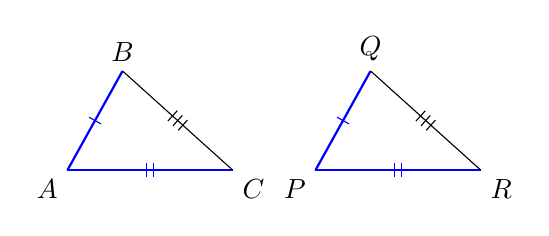
\begin{tikzpicture}[scale=0.7]
\coordinate (A) at (0,0); \coordinate (B) at (1,1.8); \coordinate (C) at (3,0);
\coordinate (P) at (4.5,0); \coordinate (Q) at (5.5,1.8); \coordinate (R) at (7.5,0);
\draw[blue,thick] (A)--(B) node[midway,sloped,inner sep=0pt] {\krastineszymek{0}} (P)--(Q) node[midway,sloped,inner sep=0pt] {\krastineszymek{0}};
\draw[blue,thick] (A)--(C) node[midway,sloped,inner sep=0pt] {\krastineszymek{-1.25,1.25}} (P)--(R) node[midway,sloped,inner sep=0pt] {\krastineszymek{-1.25,1.25}};
\draw (B)--(C) node[midway,sloped,inner sep=0pt] {\krastineszymek{-2.5,0,2.5}} (Q)--(R) node[midway,sloped,inner sep=0pt] {\krastineszymek{-2.5,0,2.5}};
\foreach \p/\pos in {A/below left,B/above,C/below right,P/below left,Q/above,R/below right} \node[\pos] at (\p) {$\p$};
\end{tikzpicture}
\end{center}
\par\emph{2 žingsnis.} Kampus $\angle ABC$ ir $\angle BAC$ atitinka $\angle PQR$ ir $\angle QPR$, o likusi kampų lygybė yra $\angle ACB=\angle PRQ$:
\begin{center}
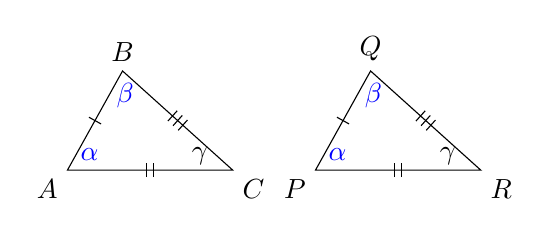
\begin{tikzpicture}[scale=0.7]
\coordinate (A) at (0,0); \coordinate (B) at (1,1.8); \coordinate (C) at (3,0);
\coordinate (P) at (4.5,0); \coordinate (Q) at (5.5,1.8); \coordinate (R) at (7.5,0);
\draw (A)--(B) node[midway,sloped,inner sep=0pt] {\krastineszymek{0}}--(C) node[midway,sloped,inner sep=0pt] {\krastineszymek{-2.5,0,2.5}}--cycle;
\draw (P)--(Q) node[midway,sloped,inner sep=0pt] {\krastineszymek{0}}--(R) node[midway,sloped,inner sep=0pt] {\krastineszymek{-2.5,0,2.5}}--cycle;
\path (A)--(C) node[midway,sloped,inner sep=0pt] {\krastineszymek{-1.25,1.25}} (P)--(R) node[midway,sloped,inner sep=0pt] {\krastineszymek{-1.25,1.25}};
\node[blue] at (0.4,0.28) {$\alpha$}; \node[blue] at (4.9,0.28) {$\alpha$};
\node[blue] at (1.05,1.35) {$\beta$}; \node[blue] at (5.55,1.35) {$\beta$};
\node at (2.4,0.25) {$\gamma$}; \node at (6.9,0.25) {$\gamma$};
\foreach \p/\pos in {A/below left,B/above,C/below right,P/below left,Q/above,R/below right} \node[\pos] at (\p) {$\p$};
\end{tikzpicture}
\end{center}
\end{solution}

\begin{solution}[\ref{uzd:lygybe-sas-01}]
\par\emph{1 žingsnis.} Duota $AB=FE$ ir $AC=FD$:
\begin{center}
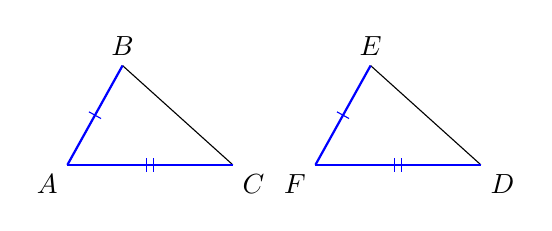
\begin{tikzpicture}[scale=0.7]
\coordinate (A) at (0,0); \coordinate (B) at (1,1.8); \coordinate (C) at (3,0);
\coordinate (F) at (4.5,0); \coordinate (E) at (5.5,1.8); \coordinate (D) at (7.5,0);
\draw (B)--(C) (E)--(D);
\draw[blue,thick] (A)--(B) node[midway,sloped,inner sep=0pt] {\krastineszymek{0}} (F)--(E) node[midway,sloped,inner sep=0pt] {\krastineszymek{0}};
\draw[blue,thick] (A)--(C) node[midway,sloped,inner sep=0pt] {\krastineszymek{-1.25,1.25}} (F)--(D) node[midway,sloped,inner sep=0pt] {\krastineszymek{-1.25,1.25}};
\foreach \p/\pos in {A/below left,B/above,C/below right,F/below left,E/above,D/below right} \node[\pos] at (\p) {$\p$};
\end{tikzpicture}
\end{center}
\par\emph{2 žingsnis.} Duota $\angle BAC=\angle EFD$ (kampai tarp tų kraštinių). Todėl $\triangle ABC=\triangle FED$ pagal dvi kraštines ir kampą tarp jų, ir iš čia $BC=ED$:
\begin{center}
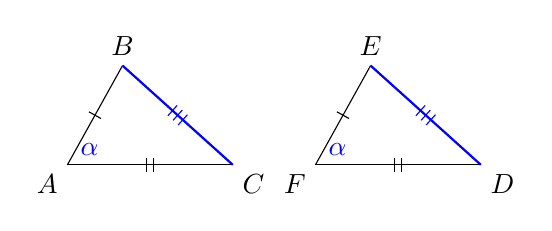
\begin{tikzpicture}[scale=0.7]
\coordinate (A) at (0,0); \coordinate (B) at (1,1.8); \coordinate (C) at (3,0);
\coordinate (F) at (4.5,0); \coordinate (E) at (5.5,1.8); \coordinate (D) at (7.5,0);
\draw (A)--(B) node[midway,sloped,inner sep=0pt] {\krastineszymek{0}} (F)--(E) node[midway,sloped,inner sep=0pt] {\krastineszymek{0}};
\draw (A)--(C) node[midway,sloped,inner sep=0pt] {\krastineszymek{-1.25,1.25}} (F)--(D) node[midway,sloped,inner sep=0pt] {\krastineszymek{-1.25,1.25}};
\draw[blue,thick] (B)--(C) node[midway,sloped,inner sep=0pt] {\krastineszymek{-2.5,0,2.5}} (E)--(D) node[midway,sloped,inner sep=0pt] {\krastineszymek{-2.5,0,2.5}};
\node[blue] at (0.4,0.28) {$\alpha$}; \node[blue] at (4.9,0.28) {$\alpha$};
\foreach \p/\pos in {A/below left,B/above,C/below right,F/below left,E/above,D/below right} \node[\pos] at (\p) {$\p$};
\end{tikzpicture}
\end{center}
\end{solution}

\begin{solution}[\ref{uzd:lygybe-asa-01}]
\par\emph{1 žingsnis.} Duota $AB=KL$:
\begin{center}
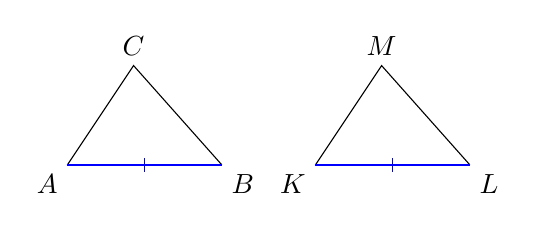
\begin{tikzpicture}[scale=0.7]
\coordinate (A) at (0,0); \coordinate (B) at (2.8,0); \coordinate (C) at (1.2,1.8);
\coordinate (K) at (4.5,0); \coordinate (L) at (7.3,0); \coordinate (M) at (5.7,1.8);
\draw (A)--(C)--(B) (K)--(M)--(L);
\draw[blue,thick] (A)--(B) node[midway,sloped,inner sep=0pt] {\krastineszymek{0}} (K)--(L) node[midway,sloped,inner sep=0pt] {\krastineszymek{0}};
\foreach \p/\pos in {A/below left,B/below right,C/above,K/below left,L/below right,M/above} \node[\pos] at (\p) {$\p$};
\end{tikzpicture}
\end{center}
\par\emph{2 žingsnis.} Duota $\angle BAC=\angle LKM$ ir $\angle ABC=\angle KLM$ (kampai prie lygių kraštinių). Todėl $\triangle ABC=\triangle KLM$ pagal kraštinę ir du kampus prie jos, taigi kraštinę $AC$ atitinka ir jai lygi yra $KM$:
\begin{center}
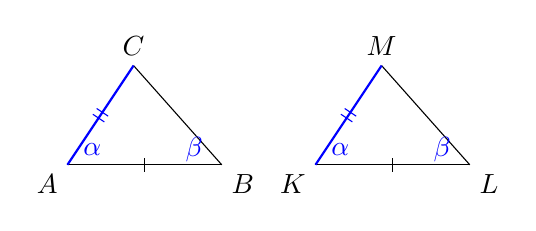
\begin{tikzpicture}[scale=0.7]
\coordinate (A) at (0,0); \coordinate (B) at (2.8,0); \coordinate (C) at (1.2,1.8);
\coordinate (K) at (4.5,0); \coordinate (L) at (7.3,0); \coordinate (M) at (5.7,1.8);
\draw (A)--(B) node[midway,sloped,inner sep=0pt] {\krastineszymek{0}} (K)--(L) node[midway,sloped,inner sep=0pt] {\krastineszymek{0}};
\draw (B)--(C) (L)--(M);
\draw[blue,thick] (A)--(C) node[midway,sloped,inner sep=0pt] {\krastineszymek{-1.25,1.25}} (K)--(M) node[midway,sloped,inner sep=0pt] {\krastineszymek{-1.25,1.25}};
\node[blue] at (0.45,0.28) {$\alpha$}; \node[blue] at (4.95,0.28) {$\alpha$};
\node[blue] at (2.3,0.28) {$\beta$}; \node[blue] at (6.8,0.28) {$\beta$};
\foreach \p/\pos in {A/below left,B/below right,C/above,K/below left,L/below right,M/above} \node[\pos] at (\p) {$\p$};
\end{tikzpicture}
\end{center}
\end{solution}

\begin{solution}[\ref{uzd:lygybe-klaida-01}]
\par\emph{1 žingsnis.} Pažymėjus $AB=DE$, $AC=DF$ ir $\angle ABC=\angle DEF$, matome, kad kampas $\angle ABC$ nėra tarp kraštinių $AB$ ir $AC$:
\begin{center}
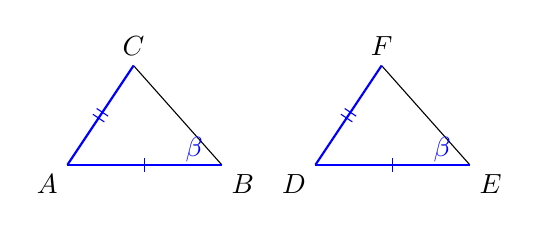
\begin{tikzpicture}[scale=0.7]
\coordinate (A) at (0,0); \coordinate (B) at (2.8,0); \coordinate (C) at (1.2,1.8);
\coordinate (D) at (4.5,0); \coordinate (E) at (7.3,0); \coordinate (F) at (5.7,1.8);
\draw (B)--(C) (E)--(F);
\draw[blue,thick] (A)--(B) node[midway,sloped,inner sep=0pt] {\krastineszymek{0}} (D)--(E) node[midway,sloped,inner sep=0pt] {\krastineszymek{0}};
\draw[blue,thick] (A)--(C) node[midway,sloped,inner sep=0pt] {\krastineszymek{-1.25,1.25}} (D)--(F) node[midway,sloped,inner sep=0pt] {\krastineszymek{-1.25,1.25}};
\node[blue] at (2.3,0.28) {$\beta$}; \node[blue] at (6.8,0.28) {$\beta$};
\foreach \p/\pos in {A/below left,B/below right,C/above,D/below left,E/below right,F/above} \node[\pos] at (\p) {$\p$};
\end{tikzpicture}
\end{center}
\par\emph{2 žingsnis.} Tarp kraštinių $AB$ ir $AC$ yra kampas $\angle BAC$. Todėl papildomai žinant $\angle BAC=\angle EDF$, pirmąjį požymį taikyti jau galima:
\begin{center}
\begin{tikzpicture}[scale=0.7]
\coordinate (A) at (0,0); \coordinate (B) at (2.8,0); \coordinate (C) at (1.2,1.8);
\coordinate (D) at (4.5,0); \coordinate (E) at (7.3,0); \coordinate (F) at (5.7,1.8);
\draw (B)--(C) (E)--(F);
\draw (A)--(B) node[midway,sloped,inner sep=0pt] {\krastineszymek{0}} (D)--(E) node[midway,sloped,inner sep=0pt] {\krastineszymek{0}};
\draw (A)--(C) node[midway,sloped,inner sep=0pt] {\krastineszymek{-1.25,1.25}} (D)--(F) node[midway,sloped,inner sep=0pt] {\krastineszymek{-1.25,1.25}};
\node at (2.3,0.28) {$\beta$}; \node at (6.8,0.28) {$\beta$};
\node[blue] at (0.45,0.28) {$\alpha$}; \node[blue] at (4.95,0.28) {$\alpha$};
\foreach \p/\pos in {A/below left,B/below right,C/above,D/below left,E/below right,F/above} \node[\pos] at (\p) {$\p$};
\end{tikzpicture}
\end{center}
\end{solution}

\begin{solution}[\ref{uzd:lygybe-ssa-01}]
\par\emph{1 žingsnis.} Trikampiuose $ABC$ ir $ABD$ pagal konstrukciją $AC=AD$:
\begin{center}
\begin{tikzpicture}[scale=.75]
\coordinate (A) at (1.2,2);\coordinate (C) at (0,0);\coordinate (D) at (2.4,0);\coordinate (B) at (4.6,0);
\draw (C)--(B) (A)--(B);
\draw[blue,thick] (A)--(C) node[midway,sloped,inner sep=0pt] {\krastineszymek{0}} (A)--(D) node[midway,sloped,inner sep=0pt] {\krastineszymek{0}};
\foreach \p/\pos in {A/above,C/below left,D/below,B/below right} {\fill (\p) circle (1.6pt) node[\pos] {$\p$};}
\end{tikzpicture}
\end{center}
\par\emph{2 žingsnis.} Kraštinė $AB$ abiem trikampiams yra bendra, o $\angle ABC=\angle ABD$ yra tas pats kampas prie viršūnės $B$:
\begin{center}
\begin{tikzpicture}[scale=.75]
\coordinate (A) at (1.2,2);\coordinate (C) at (0,0);\coordinate (D) at (2.4,0);\coordinate (B) at (4.6,0);
\draw (C)--(B) (A)--(C) node[midway,sloped,inner sep=0pt] {\krastineszymek{0}} (A)--(D) node[midway,sloped,inner sep=0pt] {\krastineszymek{0}};
\draw[blue,thick] (A)--(B) node[midway,sloped,inner sep=0pt] {\krastineszymek{-1.25,1.25}};
\node[blue] at (3.9,0.22) {$\beta$};
\foreach \p/\pos in {A/above,C/below left,D/below,B/below right} {\fill (\p) circle (1.6pt) node[\pos] {$\p$};}
\end{tikzpicture}
\end{center}
\par\emph{3 žingsnis.} Tačiau taškas $D$ yra tarp $C$ ir $B$, todėl $BC=BD+DC>BD$. Atitinkamos kraštinės $BC$ ir $BD$ nelygios, vadinasi, $\triangle ABC\ne\triangle ABD$. Dviejų kraštinių ir ne tarp jų esančio kampo lygybės nepakanka.
\end{solution}

\begin{solution}[\ref{uzd:lygybe-susikirtimas-01}]
\par\emph{1 žingsnis.} Duota $AO=OC$ ir $BO=OD$, o $\angle AOB=\angle COD$ kaip kryžminiai kampai. Todėl $\triangle AOB=\triangle COD$ pagal dvi kraštines ir kampą tarp jų; iš čia $AB=CD$, $\angle ABO=\angle CDO$ ir $\angle BAO=\angle DCO$:
\begin{center}
\begin{tikzpicture}[scale=0.75]
\coordinate (O) at (0,0); \coordinate (A) at (-2,0); \coordinate (C) at (2,0); \coordinate (B) at (-.8,-1.2); \coordinate (D) at (.8,1.2);
\fill[blue!10] (A)--(O)--(B)--cycle (C)--(O)--(D)--cycle;
\draw (A)--(C) (B)--(D) (A)--(D) (B)--(C);
\draw[blue,thick] (A)--(B) node[midway,sloped,inner sep=0pt] {\krastineszymek{-2.5,0,2.5}} (C)--(D) node[midway,sloped,inner sep=0pt] {\krastineszymek{-2.5,0,2.5}};
\path (A)--(O) node[midway,sloped,inner sep=0pt] {\krastineszymek{0}} (O)--(C) node[midway,sloped,inner sep=0pt] {\krastineszymek{0}}
      (B)--(O) node[midway,sloped,inner sep=0pt] {\krastineszymek{-1.25,1.25}} (O)--(D) node[midway,sloped,inner sep=0pt] {\krastineszymek{-1.25,1.25}};
\foreach \p/\pos in {A/left,B/below,D/above,C/right,O/below right} {\fill (\p) circle (1.6pt) node[\pos] {$\p$};}
\end{tikzpicture}
\end{center}
\par\emph{2 žingsnis.} Kryžminiai kampai $\angle AOD$ ir $\angle COB$ lygūs, todėl $\triangle AOD=\triangle COB$ pagal dvi kraštines ir kampą tarp jų; iš čia $AD=CB$:
\begin{center}
\begin{tikzpicture}[scale=0.75]
\coordinate (O) at (0,0); \coordinate (A) at (-2,0); \coordinate (C) at (2,0); \coordinate (B) at (-.8,-1.2); \coordinate (D) at (.8,1.2);
\fill[blue!10] (A)--(O)--(D)--cycle (C)--(O)--(B)--cycle;
\draw (A)--(C) (B)--(D) (A)--(B) (C)--(D);
\draw[blue,thick] (A)--(D) (B)--(C);
\path (A)--(O) node[midway,sloped,inner sep=0pt] {\krastineszymek{0}} (O)--(C) node[midway,sloped,inner sep=0pt] {\krastineszymek{0}}
      (B)--(O) node[midway,sloped,inner sep=0pt] {\krastineszymek{-1.25,1.25}} (O)--(D) node[midway,sloped,inner sep=0pt] {\krastineszymek{-1.25,1.25}};
\foreach \p/\pos in {A/left,B/below,D/above,C/right,O/below right} {\fill (\p) circle (1.6pt) node[\pos] {$\p$};}
\end{tikzpicture}
\end{center}
\par\emph{3 žingsnis.} Kadangi $O$ yra atkarpoje $BD$, tai $\angle ABD=\angle ABO=\angle CDO=\angle CDB$. Be to, $AB=CD$ ir $BD$ bendra, todėl $\triangle ABD=\triangle CDB$ pagal dvi kraštines ir kampą tarp jų. Analogiškai dėl bendros $AC$ ir $\angle BAC=\angle DCA$ gauname $\triangle BAC=\triangle DCA$:
\begin{center}
\begin{tikzpicture}[scale=0.75]
\coordinate (O) at (0,0); \coordinate (A) at (-2,0); \coordinate (C) at (2,0); \coordinate (B) at (-.8,-1.2); \coordinate (D) at (.8,1.2);
\draw (A)--(C) (A)--(D) (B)--(C);
\draw[blue,thick] (A)--(B) node[midway,sloped,inner sep=0pt] {\krastineszymek{0}} (C)--(D) node[midway,sloped,inner sep=0pt] {\krastineszymek{0}} (B)--(D);
\node[blue] at (-0.85,-0.82) {$\beta$}; \node[blue] at (0.85,0.82) {$\beta$};
\foreach \p/\pos in {A/left,B/below,D/above,C/right,O/below right} {\fill (\p) circle (1.6pt) node[\pos] {$\p$};}
\end{tikzpicture}
\end{center}
\end{solution}

\begin{solution}[\ref{uzd:lygybe-pusiaukampine-01}]
\par\emph{1 žingsnis.} Duota $AB=AC$ ir pusiaukampinė $AD$ ($\angle BAD=\angle DAC$):
\begin{center}
\begin{tikzpicture}[scale=0.75]
\coordinate (A) at (1.5,2.2); \coordinate (B) at (0,0); \coordinate (C) at (3,0); \coordinate (D) at (1.5,0);
\draw (B)--(C) (A)--(D);
\draw[blue,thick] (A)--(B) node[midway,sloped,inner sep=0pt] {\krastineszymek{0}} (A)--(C) node[midway,sloped,inner sep=0pt] {\krastineszymek{0}};
\node[blue] at (1.28,1.65) {$\alpha$}; \node[blue] at (1.72,1.65) {$\alpha$};
\foreach \p/\pos in {A/above,B/below left,C/below right,D/below} {\fill (\p) circle (1.6pt) node[\pos] {$\p$};}
\end{tikzpicture}
\end{center}
\par\emph{2 žingsnis.} Kraštinė $AD$ yra bendra, todėl $\triangle BAD=\triangle CAD$ pagal dvi kraštines ir kampą tarp jų:
\begin{center}
\begin{tikzpicture}[scale=0.75]
\coordinate (A) at (1.5,2.2); \coordinate (B) at (0,0); \coordinate (C) at (3,0); \coordinate (D) at (1.5,0);
\fill[blue!10] (A)--(B)--(D)--cycle (A)--(C)--(D)--cycle;
\draw (B)--(C) (A)--(B) node[midway,sloped,inner sep=0pt] {\krastineszymek{0}} (A)--(C) node[midway,sloped,inner sep=0pt] {\krastineszymek{0}};
\draw[blue,thick] (A)--(D) node[midway,sloped,inner sep=0pt] {\krastineszymek{-1.25,1.25}};
\node at (1.28,1.65) {$\alpha$}; \node at (1.72,1.65) {$\alpha$};
\foreach \p/\pos in {A/above,B/below left,C/below right,D/below} {\fill (\p) circle (1.6pt) node[\pos] {$\p$};}
\end{tikzpicture}
\end{center}
\par\emph{3 žingsnis.} Iš trikampių lygumo gauname $BD=DC$ ir gretutinių kampų lygybę $\angle ADB=\angle ADC=90^\circ$, t.\,y. $AD\perp BC$:
\begin{center}
\begin{tikzpicture}[scale=0.75]
\coordinate (A) at (1.5,2.2); \coordinate (B) at (0,0); \coordinate (C) at (3,0); \coordinate (D) at (1.5,0);
\draw (A)--(B) node[midway,sloped,inner sep=0pt] {\krastineszymek{0}} (A)--(C) node[midway,sloped,inner sep=0pt] {\krastineszymek{0}} (A)--(D);
\draw[blue,thick] (B)--(D) node[midway,sloped,inner sep=0pt] {\krastineszymek{-1.25,1.25}} (D)--(C) node[midway,sloped,inner sep=0pt] {\krastineszymek{-1.25,1.25}};
\draw[blue,thick] (1.5,0.25)--(1.75,0.25)--(1.75,0);
\node at (1.28,1.65) {$\alpha$}; \node at (1.72,1.65) {$\alpha$};
\foreach \p/\pos in {A/above,B/below left,C/below right,D/below} {\fill (\p) circle (1.6pt) node[\pos] {$\p$};}
\end{tikzpicture}
\end{center}
\end{solution}

\begin{solution}[\ref{uzd:lygias-supratimas-01}]
Pagrindas yra $BC$, o kampai prie jo – $\angle ABC$ ir $\angle BCA$. Jei lygios visos kraštinės, tai lygios ir bet kurios dvi iš jų, todėl trikampis atitinka lygiašonio trikampio apibrėžimą, o pagrindu galima laikyti bet kurią kraštinę.
\end{solution}

\begin{solution}[\ref{uzd:lygias-perimetras-01}]
\par\emph{1 atvejis.} Jei $6$ cm ilgio kraštinė yra pagrindas, tai abi šoninės kraštinės lygios $(20-6):2=7$ cm ($6<7+7$).
\par\emph{2 atvejis.} Jei $6$ cm ilgio kraštinė yra šoninė, tai kita šoninė kraštinė irgi lygi $6$ cm, o pagrindas lygus $20-6-6=8$ cm ($8<6+6$):
\begin{center}
\begin{tikzpicture}[scale=0.65]
\draw (0,0)--(2,0) node[midway,below] {$6$}--(1,2.1) node[midway,right] {$7$}--cycle node[midway,left] {$7$};
\draw (4.5,0)--(7.3,0) node[midway,below] {$8$}--(5.9,1.7) node[midway,right] {$6$}--cycle node[midway,left] {$6$};
\end{tikzpicture}
\end{center}
\end{solution}

\begin{solution}[\ref{atr:lygias-pagrindo-kampai}]
\par\emph{1 žingsnis.} Duotas lygiašonis trikampis, kurio $AB=AC$:
\begin{center}
\begin{tikzpicture}[scale=0.75]
\coordinate (A) at (1.5,2.2); \coordinate (B) at (0,0); \coordinate (C) at (3,0);
\draw (B)--(C);
\draw[blue,thick] (A)--(B) node[midway,sloped,inner sep=0pt] {\krastineszymek{0}} (A)--(C) node[midway,sloped,inner sep=0pt] {\krastineszymek{0}};
\foreach \p/\pos in {A/above,B/below left,C/below right} {\fill (\p) circle (1.6pt) node[\pos] {$\p$};}
\end{tikzpicture}
\end{center}
\par\emph{2 žingsnis.} Nubrėžiame kampo $BAC$ pusiaukampinę $AD$ ($\angle BAD=\angle CAD$), kuri kerta $BC$ taške $D$:
\begin{center}
\begin{tikzpicture}[scale=0.75]
\coordinate (A) at (1.5,2.2); \coordinate (B) at (0,0); \coordinate (C) at (3,0); \coordinate (D) at (1.5,0);
\draw (B)--(C) (A)--(B) node[midway,sloped,inner sep=0pt] {\krastineszymek{0}} (A)--(C) node[midway,sloped,inner sep=0pt] {\krastineszymek{0}};
\draw[blue,thick] (A)--(D);
\node[blue] at (1.28,1.65) {$\alpha$}; \node[blue] at (1.72,1.65) {$\alpha$};
\foreach \p/\pos in {A/above,B/below left,C/below right,D/below} {\fill (\p) circle (1.6pt) node[\pos] {$\p$};}
\end{tikzpicture}
\end{center}
\par\emph{3 žingsnis.} Kadangi $AD$ bendra, $\triangle BAD=\triangle CAD$ pagal dvi kraštines ir kampą tarp jų, todėl atitinkami kampai prie pagrindo lygūs: $\angle ABC=\angle ACB$:
\begin{center}
\begin{tikzpicture}[scale=0.75]
\coordinate (A) at (1.5,2.2); \coordinate (B) at (0,0); \coordinate (C) at (3,0); \coordinate (D) at (1.5,0);
\draw (B)--(C) (A)--(B) node[midway,sloped,inner sep=0pt] {\krastineszymek{0}} (A)--(C) node[midway,sloped,inner sep=0pt] {\krastineszymek{0}} (A)--(D) node[midway,sloped,inner sep=0pt] {\krastineszymek{-1.25,1.25}};
\node at (1.28,1.65) {$\alpha$}; \node at (1.72,1.65) {$\alpha$};
\node[blue] at (0.48,0.25) {$\beta$}; \node[blue] at (2.52,0.25) {$\beta$};
\foreach \p/\pos in {A/above,B/below left,C/below right,D/below} {\fill (\p) circle (1.6pt) node[\pos] {$\p$};}
\end{tikzpicture}
\end{center}
\end{solution}

\begin{solution}[\ref{uzd:lygias-kampai-01}]
Pagal lygiašonio trikampio kampų prie pagrindo savybę (\ref{atr:lygias-pagrindo-kampai}) $\angle ACB=\angle ABC=38^\circ$. Lygybė $AB=BC$ neišplaukia: nubraižę $38^\circ$ kampą su viršūne $B$, atidėję $BA=3$ cm ir skriestuvu radę tašką $C$, kuriam $AC=3$ cm, išmatavę gauname $BC\approx 4{,}7\text{ cm}\ne AB$.
\end{solution}

\begin{solution}[\ref{uzd:lygias-kampai-02}]
Kadangi $PQ=QR$, kampai prie pagrindo $PR$ lygūs: $2x+10=3x-5$, iš kur $x=15$. Abu kampai lygūs po $40^\circ$.
\end{solution}

\begin{solution}[\ref{atr:lygias-atvirkstine}]
\par\emph{1 žingsnis.} Duotas trikampis $ABC$, kuriame $\angle ABC=\angle BCA$:
\begin{center}
\begin{tikzpicture}[scale=0.75]
\coordinate (A) at (1.5,2.1); \coordinate (B) at (0,0); \coordinate (C) at (3,0);
\draw (A)--(B)--(C)--cycle;
\node[blue] at (0.48,0.25) {$\alpha$}; \node[blue] at (2.52,0.25) {$\alpha$};
\foreach \p/\pos in {A/above,B/below left,C/below right} {\fill (\p) circle (1.6pt) node[\pos] {$\p$};}
\end{tikzpicture}
\end{center}
\par\emph{2 žingsnis.} Palyginame trikampį $ABC$ su juo pačiu, užrašytu kita viršūnių tvarka – $\triangle ACB$. Kraštinė $BC$ bendra ($BC=CB$), o kampai prie jos poromis lygūs ($\angle ABC=\angle ACB$ ir $\angle BCA=\angle CBA$). Todėl $\triangle ABC=\triangle ACB$ pagal kraštinę ir du kampus prie jos, iš kur gauname $AB=AC$:
\begin{center}
\begin{tikzpicture}[scale=0.75]
\coordinate (A) at (1.5,2.1); \coordinate (B) at (0,0); \coordinate (C) at (3,0);
\draw (B)--(C) node[midway,sloped,inner sep=0pt] {\krastineszymek{-1.25,1.25}};
\draw[blue,thick] (A)--(B) node[midway,sloped,inner sep=0pt] {\krastineszymek{0}} (A)--(C) node[midway,sloped,inner sep=0pt] {\krastineszymek{0}};
\node at (0.48,0.25) {$\alpha$}; \node at (2.52,0.25) {$\alpha$};
\foreach \p/\pos in {A/above,B/below left,C/below right} {\fill (\p) circle (1.6pt) node[\pos] {$\p$};}
\end{tikzpicture}
\end{center}
\end{solution}

\begin{solution}[\ref{uzd:lygias-atvirkstine-01}]
Pagal lygiašonio trikampio požymį (\ref{atr:lygias-atvirkstine}) iš $\angle ABC=\angle BCA$ gauname $AC=AB=7$ cm.
\end{solution}

\begin{solution}[\ref{uzd:lygias-atvirkstine-02}]
Prieš lygius kampus $\angle KLM$ ir $\angle LKM$ yra kraštinės $KM$ ir $LM$, todėl pagal lygiašonio trikampio požymį $KM=LM$. Kampai $K$ ir $M$ nebūtinai lygūs: paėmę $KL=4$ cm ir prie $K$ bei $L$ atidėję po $30^\circ$ kampus, gauname $LM\approx 2{,}3\text{ cm}\ne KL$.
\end{solution}

\begin{solution}[\ref{atr:lygias-pusiaukrastine}]
\par\emph{1 žingsnis.} Duota $AB=AC$ ir $BM=MC$:
\begin{center}
\begin{tikzpicture}[scale=0.75]
\coordinate (A) at (1.5,2.2); \coordinate (B) at (0,0); \coordinate (C) at (3,0); \coordinate (M) at (1.5,0);
\draw (A)--(M);
\draw[blue,thick] (A)--(B) node[midway,sloped,inner sep=0pt] {\krastineszymek{0}} (A)--(C) node[midway,sloped,inner sep=0pt] {\krastineszymek{0}};
\draw[blue,thick] (B)--(M) node[midway,sloped,inner sep=0pt] {\krastineszymek{-1.25,1.25}} (M)--(C) node[midway,sloped,inner sep=0pt] {\krastineszymek{-1.25,1.25}};
\foreach \p/\pos in {A/above,B/below left,C/below right,M/below} {\fill (\p) circle (1.6pt) node[\pos] {$\p$};}
\end{tikzpicture}
\end{center}
\par\emph{2 žingsnis.} Pagal lygiašonio trikampio kampų prie pagrindo savybę (\ref{atr:lygias-pagrindo-kampai}) $\angle ABM=\angle ACM$. Todėl $\triangle ABM=\triangle ACM$ pagal dvi kraštines ir kampą tarp jų:
\begin{center}
\begin{tikzpicture}[scale=0.75]
\coordinate (A) at (1.5,2.2); \coordinate (B) at (0,0); \coordinate (C) at (3,0); \coordinate (M) at (1.5,0);
\fill[blue!10] (A)--(B)--(M)--cycle (A)--(C)--(M)--cycle;
\draw (A)--(M) (A)--(B) node[midway,sloped,inner sep=0pt] {\krastineszymek{0}} (A)--(C) node[midway,sloped,inner sep=0pt] {\krastineszymek{0}}
      (B)--(M) node[midway,sloped,inner sep=0pt] {\krastineszymek{-1.25,1.25}} (M)--(C) node[midway,sloped,inner sep=0pt] {\krastineszymek{-1.25,1.25}};
\node[blue] at (0.48,0.25) {$\beta$}; \node[blue] at (2.52,0.25) {$\beta$};
\foreach \p/\pos in {A/above,B/below left,C/below right,M/below} {\fill (\p) circle (1.6pt) node[\pos] {$\p$};}
\end{tikzpicture}
\end{center}
\par\emph{3 žingsnis.} Iš trikampių lygumo $\angle BAM=\angle MAC$ ($AM$ – pusiaukampinė) ir gretutiniai kampai $\angle AMB=\angle AMC=90^\circ$ ($AM$ – aukštinė):
\begin{center}
\begin{tikzpicture}[scale=0.75]
\coordinate (A) at (1.5,2.2); \coordinate (B) at (0,0); \coordinate (C) at (3,0); \coordinate (M) at (1.5,0);
\draw (A)--(M) (A)--(B) node[midway,sloped,inner sep=0pt] {\krastineszymek{0}} (A)--(C) node[midway,sloped,inner sep=0pt] {\krastineszymek{0}}
      (B)--(M) node[midway,sloped,inner sep=0pt] {\krastineszymek{-1.25,1.25}} (M)--(C) node[midway,sloped,inner sep=0pt] {\krastineszymek{-1.25,1.25}};
\node at (0.48,0.25) {$\beta$}; \node at (2.52,0.25) {$\beta$};
\node[blue] at (1.28,1.65) {$\alpha$}; \node[blue] at (1.72,1.65) {$\alpha$};
\draw[blue,thick] (1.5,0.25)--(1.75,0.25)--(1.75,0);
\foreach \p/\pos in {A/above,B/below left,C/below right,M/below} {\fill (\p) circle (1.6pt) node[\pos] {$\p$};}
\end{tikzpicture}
\end{center}
\end{solution}

\begin{solution}[\ref{uzd:lygias-pusiaukrastine-01}]
Pagal \ref{atr:lygias-pusiaukrastine} uždavinį pusiaukraštinė $AM$ yra ir pusiaukampinė, ir aukštinė, todėl $\angle MAC=\angle BAM=27^\circ$ ir $\angle AMB=90^\circ$.
\end{solution}

\begin{solution}[\ref{uzd:lygias-aukstine-01}]
\par\emph{1 žingsnis.} Duota $AB=AC$ ir $AD\perp BC$. Pažymėkime $BC$ vidurio tašką $M$:
\begin{center}
\begin{tikzpicture}[scale=0.75]
\coordinate (A) at (1.5,2.2); \coordinate (B) at (0,0); \coordinate (C) at (3,0); \coordinate (D) at (1.3,0); \coordinate (M) at (1.7,0);
\draw (B)--(C) (A)--(B) node[midway,sloped,inner sep=0pt] {\krastineszymek{0}} (A)--(C) node[midway,sloped,inner sep=0pt] {\krastineszymek{0}} (A)--(D);
\draw[blue,thick,dashed] (A)--(M);
\foreach \p/\pos in {A/above,B/below left,C/below right,D/below left} {\fill (\p) circle (1.6pt) node[\pos] {$\p$};}
\fill[blue] (M) circle (1.6pt) node[below right,blue] {$M$};
\end{tikzpicture}
\end{center}
\par\emph{2 žingsnis.} Pagal lygiašonio trikampio pusiaukraštinės savybę (\ref{atr:lygias-pusiaukrastine}) $AM\perp BC$. Kadangi per tašką $A$ eina tik viena tiesei $BC$ statmena tiesė, tiesės $AM$ ir $AD$ sutampa, t.\,y. $D=M$. Todėl $BD=DC$ ir $\angle BAD=\angle DAC$:
\begin{center}
\begin{tikzpicture}[scale=0.75]
\coordinate (A) at (1.5,2.2); \coordinate (B) at (0,0); \coordinate (C) at (3,0); \coordinate (D) at (1.5,0);
\draw (A)--(B) node[midway,sloped,inner sep=0pt] {\krastineszymek{0}} (A)--(C) node[midway,sloped,inner sep=0pt] {\krastineszymek{0}} (A)--(D);
\draw[blue,thick] (B)--(D) node[midway,sloped,inner sep=0pt] {\krastineszymek{-1.25,1.25}} (D)--(C) node[midway,sloped,inner sep=0pt] {\krastineszymek{-1.25,1.25}};
\draw (1.5,0.25)--(1.75,0.25)--(1.75,0);
\node[blue] at (1.28,1.65) {$\alpha$}; \node[blue] at (1.72,1.65) {$\alpha$};
\foreach \p/\pos in {A/above,B/below left,C/below right} {\fill (\p) circle (1.6pt) node[\pos] {$\p$};}
\fill[blue] (D) circle (1.6pt) node[below,blue] {$D=M$};
\end{tikzpicture}
\end{center}
\end{solution}

\begin{solution}[\ref{uzd:lygias-pusiaukampines-01}]
\par\emph{1 žingsnis.} Duota $AB=AC$, todėl pagal kampų prie pagrindo savybę $\angle ABC=\angle ACB$:
\begin{center}
\begin{tikzpicture}[scale=0.75]
\coordinate (A) at (1.5,2.5); \coordinate (B) at (0,0); \coordinate (C) at (3,0);
\draw (B)--(C) (A)--(B) node[midway,sloped,inner sep=0pt] {\krastineszymek{0}} (A)--(C) node[midway,sloped,inner sep=0pt] {\krastineszymek{0}};
\node[blue] at (0.45,0.25) {$2\alpha$}; \node[blue] at (2.55,0.25) {$2\alpha$};
\foreach \p/\pos in {A/above,B/below left,C/below right} {\fill (\p) circle (1.6pt) node[\pos] {$\p$};}
\end{tikzpicture}
\end{center}
\par\emph{2 žingsnis.} Nubrėžus pusiaukampines $BD$ ir $CE$, lygių kampų pusės taip pat lygios: $\angle DBC=\angle ECB=\alpha$:
\begin{center}
\begin{tikzpicture}[scale=0.75]
\coordinate (A) at (1.5,2.5); \coordinate (B) at (0,0); \coordinate (C) at (3,0);
\coordinate (D) at (2.35,1.08); \coordinate (E) at (0.65,1.08);
\draw (B)--(C) (A)--(B) (A)--(C);
\draw[blue,thick] (B)--(D) (C)--(E);
\node[blue] at (0.65,0.18) {$\alpha$}; \node[blue] at (2.35,0.18) {$\alpha$};
\foreach \p/\pos in {A/above,B/below left,C/below right,D/right,E/left} {\fill (\p) circle (1.6pt) node[\pos] {$\p$};}
\end{tikzpicture}
\end{center}
\par\emph{3 žingsnis.} Trikampiuose $DBC$ ir $ECB$ kraštinė $BC$ yra bendra, $\angle DBC=\angle ECB$ ir $\angle DCB=\angle EBC$. Todėl $\triangle DBC=\triangle ECB$ pagal kraštinę ir du kampus prie jos, iš kur $BD=CE$:
\begin{center}
\begin{tikzpicture}[scale=0.75]
\coordinate (A) at (1.5,2.5); \coordinate (B) at (0,0); \coordinate (C) at (3,0);
\coordinate (D) at (2.35,1.08); \coordinate (E) at (0.65,1.08);
\fill[blue!10] (D)--(B)--(C)--cycle (E)--(C)--(B)--cycle;
\draw (A)--(B) (A)--(C) (B)--(D) (C)--(E);
\draw[blue,thick] (B)--(C) node[midway,sloped,inner sep=0pt] {\krastineszymek{-1.25,1.25}};
\node at (0.65,0.18) {$\alpha$}; \node at (2.35,0.18) {$\alpha$};
\foreach \p/\pos in {A/above,B/below left,C/below right,D/right,E/left} {\fill (\p) circle (1.6pt) node[\pos] {$\p$};}
\end{tikzpicture}
\end{center}
\end{solution}

\begin{solution}[\ref{uzd:lygiakrastis-supratimas-01}]
Taip, kiekvienas lygiakraštis trikampis turi bent dvi lygias kraštines, todėl yra lygiašonis. Ne kiekvienas lygiašonis trikampis yra lygiakraštis (pvz., trikampis su kraštinėmis $7$, $7$, $6$ cm).
\end{solution}

\begin{solution}[\ref{atr:lygiakrastis-kampai}]
\par\emph{1 žingsnis.} Jei $AB=BC=CA$, tai iš $AB=AC$ gauname $\angle B=\angle C$, o iš $BA=BC$ gauname $\angle A=\angle C$, todėl visi kampai lygūs:
\begin{center}
\begin{tikzpicture}[scale=0.7]
\coordinate (A) at (1.5,2.6); \coordinate (B) at (0,0); \coordinate (C) at (3,0);
\draw (A)--(B) node[midway,sloped,inner sep=0pt] {\krastineszymek{0}}--(C) node[midway,sloped,inner sep=0pt] {\krastineszymek{0}}--cycle node[midway,sloped,inner sep=0pt] {\krastineszymek{0}};
\node[blue] at (0.55,0.28) {$\alpha$}; \node[blue] at (2.45,0.28) {$\alpha$}; \node[blue] at (1.5,2.05) {$\alpha$};
\foreach \p/\pos in {A/above,B/below left,C/below right} {\fill (\p) circle (1.6pt) node[\pos] {$\p$};}
\end{tikzpicture}
\end{center}
\par\emph{2 žingsnis.} Atvirkščiai, jei $\angle A=\angle B=\angle C$, tai pagal lygiašonio trikampio požymį iš $\angle B=\angle C$ išplaukia $AB=AC$, o iš $\angle A=\angle C$ išplaukia $BC=BA$, taigi $AB=BC=CA$.
\end{solution}

\begin{solution}[\ref{uzd:lygiakrastis-kampai-01}]
Pagal lygiakraščio trikampio savybę (\ref{atr:lygiakrastis-kampai}) $\angle BAC=\angle BCA$. Vien iš jų lygybės negalime teigti, kad jie lygūs $60^\circ$, nes šiame lape nenaudojame fakto apie trikampio kampų sumą.
\end{solution}

\begin{solution}[\ref{atr:sss-poz}]
\textbf{a)}
\par\emph{1 žingsnis.} Kitoje tiesės $AC$ pusėje nei $B$ atidedame $\angle CAK=\angle EDF$ ir $AK=DF$, nubrėžiame $KC$:
\begin{center}
\begin{tikzpicture}[scale=0.7]
\coordinate (A) at (0,0);\coordinate (B) at (1.5,1.6);\coordinate (C) at (3.6,0);\coordinate (K) at (1.5,-1.6);
\draw (A)--(B) node[midway,sloped,inner sep=0pt] {\krastineszymek{0}}--(C) node[midway,sloped,inner sep=0pt] {\krastineszymek{-1.25,1.25}}--cycle node[midway,sloped,inner sep=0pt] {\krastineszymek{-2.5,0,2.5}};
\draw[blue,thick] (A)--(K) node[midway,sloped,inner sep=0pt] {\krastineszymek{0}}--(C);
\node[blue] at (0.5,-0.25) {$\alpha$};
\foreach \p/\pos in {A/left,B/above,C/right,K/below} {\fill (\p) circle (1.6pt) node[\pos] {$\p$};}
\end{tikzpicture}
\end{center}
\par\emph{2 žingsnis.} Kadangi $AK=DF$, $AC=DE$ ir $\angle CAK=\angle EDF$, tai $\triangle AKC=\triangle DFE$ pagal dvi kraštines ir kampą tarp jų. Todėl $CK=FE=CB$ ir $AK=DF=AB$:
\begin{center}
\begin{tikzpicture}[scale=0.7]
\coordinate (A) at (0,0);\coordinate (B) at (1.5,1.6);\coordinate (C) at (3.6,0);\coordinate (K) at (1.5,-1.6);
\draw (A)--(B) node[midway,sloped,inner sep=0pt] {\krastineszymek{0}}--(C) node[midway,sloped,inner sep=0pt] {\krastineszymek{-1.25,1.25}} (A)--(K) node[midway,sloped,inner sep=0pt] {\krastineszymek{0}};
\draw (A)--(C) node[midway,sloped,inner sep=0pt] {\krastineszymek{-2.5,0,2.5}};
\draw[blue,thick] (K)--(C) node[midway,sloped,inner sep=0pt] {\krastineszymek{-1.25,1.25}};
\draw[blue,dashed] (B)--(K);
\foreach \p/\pos in {A/left,B/above,C/right,K/below} {\fill (\p) circle (1.6pt) node[\pos] {$\p$};}
\end{tikzpicture}
\end{center}

\textbf{b)} Trikampiai $ABK$ ir $CBK$ yra lygiašoniai su bendru pagrindu $BK$, todėl $\angle ABK=\angle AKB=\alpha$ ir $\angle CBK=\angle CKB=\beta$:
\begin{center}
\begin{tikzpicture}[scale=.48,font=\small]
\coordinate (A) at (0,0);\coordinate (C) at (4,0);\coordinate (B) at (1.5,1.8);\coordinate (K) at (1.5,-1.8);\coordinate (X) at (1.5,0);
\draw (A)--(B)--(C)--(K)--cycle (A)--(C); \draw[blue,thick] (B)--(K);
\node[blue] at (1.2,1.1) {$\alpha$}; \node[blue] at (1.2,-1.1) {$\alpha$};
\node[blue] at (1.85,1.1) {$\beta$}; \node[blue] at (1.85,-1.1) {$\beta$};
\foreach \p/\pos in {A/left,B/above,C/right,K/below,X/above right} {\fill (\p) circle (1.6pt) node[\pos] {$\p$};}
\node at (2,-2.8) {1 atvejis: $\alpha+\beta$};
\end{tikzpicture}\hspace{1em}
\begin{tikzpicture}[scale=.48,font=\small]
\coordinate (A) at (0,0);\coordinate (C) at (3.5,0);\coordinate (B) at (0,1.8);\coordinate (K) at (0,-1.8);
\draw (A)--(B)--(C)--(K)--cycle (A)--(C); \draw[blue,thick] (B)--(K);
\node[blue] at (0.4,1.1) {$\beta$}; \node[blue] at (0.4,-1.1) {$\beta$};
\foreach \p/\pos in {B/above,C/right,K/below} {\fill (\p) circle (1.6pt) node[\pos] {$\p$};}
\fill (A) circle (1.6pt) node[left] {$A=X$};
\node at (1.75,-2.8) {2 atvejis: $\beta=\beta$};
\end{tikzpicture}\hspace{1em}
\begin{tikzpicture}[scale=.48,font=\small]
\coordinate (A) at (0,0);\coordinate (C) at (3.5,0);\coordinate (B) at (-1,1.8);\coordinate (K) at (-1,-1.8);\coordinate (X) at (-1,0);
\draw (A)--(B)--(C)--(K)--cycle (A)--(C); \draw[blue,thick] (B)--(K); \draw[dashed] (X)--(A);
\node[blue] at (-0.75,1.0) {$\alpha$}; \node[blue] at (-0.75,-1.0) {$\alpha$};
\node[blue] at (-0.2,1.25) {$\beta$}; \node[blue] at (-0.2,-1.25) {$\beta$};
\foreach \p/\pos in {A/above right,B/above,C/right,K/below,X/left} {\fill (\p) circle (1.6pt) node[\pos] {$\p$};}
\node at (1.25,-2.8) {3 atvejis: $\beta-\alpha$};
\end{tikzpicture}
\end{center}
Visais trimis atvejais ($\angle ABC=\alpha+\beta$, $\angle ABC=\beta$ arba $\angle ABC=\beta-\alpha$) gauname $\angle ABC=\angle AKC$.

\textbf{c)} Kadangi $AB=AK$, $BC=KC$ ir $\angle ABC=\angle AKC$, tai $\triangle ABC=\triangle AKC$ pagal dvi kraštines ir kampą tarp jų. Kartu su a) dalimi ($\triangle AKC=\triangle DFE$) gauname $\triangle ABC=\triangle DFE$.
\end{solution}

\begin{solution}[\ref{uzd:sss-breziniai-01}]
\textbf{(1)} Duota $AB=AD$ ir $CB=CD$, o kraštinė $AC$ yra bendra (pridedame tris brūkšnelius). Todėl $\triangle ABC=\triangle ADC$ pagal tris kraštines:
\begin{center}
\begin{tikzpicture}[scale=.75]
\coordinate (A) at (0,0);\coordinate (C) at (4,0);\coordinate (B) at (1.5,1.5);\coordinate (D) at (1.5,-1.5);
\fill[blue!10] (A)--(B)--(C)--cycle (A)--(D)--(C)--cycle;
\draw (A)--(B) node[midway,sloped,inner sep=0pt] {\krastineszymek{0}}--(C) node[midway,sloped,inner sep=0pt] {\krastineszymek{-1.25,1.25}}--(D) node[midway,sloped,inner sep=0pt] {\krastineszymek{-1.25,1.25}}--cycle node[midway,sloped,inner sep=0pt] {\krastineszymek{0}};
\draw[blue,thick] (A)--(C) node[midway,sloped,inner sep=0pt] {\krastineszymek{-2.5,0,2.5}};
\foreach \p/\d in {A/left,B/above,C/right,D/below} \node[\d] at (\p) {$\p$};
\end{tikzpicture}
\end{center}

\textbf{(2)} Iš $AB=AE$, $AC=AD$ ir $BC=ED$ pagal tris kraštines gauname $\triangle ABC=\triangle AED$. Duomuo $BC=DE$ nebūtinas, nes kampas $A$ yra bendras, tad lygumas išplaukia ir pagal dvi kraštines ir kampą tarp jų (žr. \ref{uzd:breziniai-lygumas-01}(5)).

\textbf{(3)}
\par\emph{1 žingsnis.} Kadangi $B$ yra tarp $A$ ir $C$, o $E$ – tarp $D$ ir $F$, iš $AB=DE$ ir $BC=EF$ gauname pilnų kraštinių lygybę $AC=AB+BC=DE+EF=DF$:
\begin{center}
\begin{tikzpicture}[scale=.7]
\coordinate (A) at (0,0);\coordinate (B) at (1,0);\coordinate (C) at (3.5,0);\coordinate (D) at (0,2.6);\coordinate (E) at (1,2.6);\coordinate (F) at (3.5,2.6);\coordinate (G) at (.8,1.3);
\draw (A)--(G)--(C) (D)--(G)--(F);
\draw[blue,thick] (A)--(C) (D)--(F);
\path (A)--(B) node[midway,sloped,inner sep=0pt] {\krastineszymek{0}} (D)--(E) node[midway,sloped,inner sep=0pt] {\krastineszymek{0}}
      (B)--(C) node[midway,sloped,inner sep=0pt] {\krastineszymek{-1.25,1.25}} (E)--(F) node[midway,sloped,inner sep=0pt] {\krastineszymek{-1.25,1.25}};
\foreach \p/\d in {A/below left,B/below,C/below right,D/above left,E/above,F/above right,G/left} \node[\d] at (\p) {$\p$};
\end{tikzpicture}
\end{center}
\par\emph{2 žingsnis.} Pridėję duotas lygybes $AG=DG$ ir $CG=FG$, gauname $\triangle ACG=\triangle DFG$ pagal tris kraštines:
\begin{center}
\begin{tikzpicture}[scale=.7]
\coordinate (A) at (0,0);\coordinate (B) at (1,0);\coordinate (C) at (3.5,0);\coordinate (D) at (0,2.6);\coordinate (E) at (1,2.6);\coordinate (F) at (3.5,2.6);\coordinate (G) at (.8,1.3);
\fill[blue!10] (A)--(C)--(G)--cycle (D)--(F)--(G)--cycle;
\draw (A)--(C) (D)--(F);
\draw[blue,thick] (A)--(G) (D)--(G) (C)--(G) (F)--(G);
\path (A)--(B) node[midway,sloped,inner sep=0pt] {\krastineszymek{0}} (D)--(E) node[midway,sloped,inner sep=0pt] {\krastineszymek{0}}
      (B)--(C) node[midway,sloped,inner sep=0pt] {\krastineszymek{-1.25,1.25}} (E)--(F) node[midway,sloped,inner sep=0pt] {\krastineszymek{-1.25,1.25}};
\foreach \p/\d in {A/below left,B/below,C/below right,D/above left,E/above,F/above right,G/left} \node[\d] at (\p) {$\p$};
\end{tikzpicture}
\end{center}
\end{solution}

\begin{solution}[\ref{uzd:sss-tiesioginis-01}]
Iš lygybių $AB=PR$, $BC=RQ$, $CA=QP$ matome viršūnių atitikimą $A\leftrightarrow P$, $B\leftrightarrow R$, $C\leftrightarrow Q$. Todėl $\triangle ABC=\triangle PRQ$ pagal tris kraštines.
\end{solution}

\begin{solution}[\ref{uzd:sss-tiesioginis-02}]
\par\emph{1 žingsnis.} Duota $AB=CD$ ir $AD=CB$:
\begin{center}
\begin{tikzpicture}[scale=0.75]
\coordinate (A) at (-2,0); \coordinate (C) at (2,0); \coordinate (B) at (-0.8,-1.2); \coordinate (D) at (0.8,1.2);
\draw (A)--(C) (B)--(D);
\draw[blue,thick] (A)--(B) node[midway,sloped,inner sep=0pt] {\krastineszymek{0}} (C)--(D) node[midway,sloped,inner sep=0pt] {\krastineszymek{0}};
\draw[blue,thick] (A)--(D) node[midway,sloped,inner sep=0pt] {\krastineszymek{-1.25,1.25}} (B)--(C) node[midway,sloped,inner sep=0pt] {\krastineszymek{-1.25,1.25}};
\foreach \p/\pos in {A/left,B/below,D/above,C/right} {\fill (\p) circle (1.6pt) node[\pos] {$\p$};}
\end{tikzpicture}
\end{center}
\par\emph{2 žingsnis.} Kraštinė $BD$ yra bendra, todėl $\triangle BAD=\triangle DCB$ pagal tris kraštines (atitinka $B\leftrightarrow D$, $A\leftrightarrow C$, $D\leftrightarrow B$). Iš čia $\angle BAD=\angle DCB$, $\angle ABD=\angle CDB$ ir $\angle ADB=\angle CBD$:
\begin{center}
\begin{tikzpicture}[scale=0.75]
\coordinate (A) at (-2,0); \coordinate (C) at (2,0); \coordinate (B) at (-0.8,-1.2); \coordinate (D) at (0.8,1.2);
\fill[blue!10] (B)--(A)--(D)--cycle (D)--(C)--(B)--cycle;
\draw (A)--(B) node[midway,sloped,inner sep=0pt] {\krastineszymek{0}} (C)--(D) node[midway,sloped,inner sep=0pt] {\krastineszymek{0}}
      (A)--(D) node[midway,sloped,inner sep=0pt] {\krastineszymek{-1.25,1.25}} (B)--(C) node[midway,sloped,inner sep=0pt] {\krastineszymek{-1.25,1.25}};
\draw[blue,thick] (B)--(D) node[midway,sloped,inner sep=0pt] {\krastineszymek{-2.5,0,2.5}};
\node[blue] at (-1.45,0) {$\alpha$}; \node[blue] at (1.45,0) {$\alpha$};
\foreach \p/\pos in {A/left,B/below,D/above,C/right} {\fill (\p) circle (1.6pt) node[\pos] {$\p$};}
\end{tikzpicture}
\end{center}
\end{solution}

\begin{solution}[\ref{uzd:sss-konstr-01}]
\par\emph{1 žingsnis.} Kitoje tiesės $AB$ pusėje atidedame kampą $\angle BAD=\angle BAC$ ir atkarpą $AD=AC$:
\begin{center}
\begin{tikzpicture}[scale=0.75]
\coordinate (A) at (0,0); \coordinate (B) at (3,0); \coordinate (C) at (1.2,1.5); \coordinate (D) at (1.2,-1.5);
\draw (A)--(B) (B)--(C) (A)--(C) node[midway,sloped,inner sep=0pt] {\krastineszymek{0}};
\draw[blue,thick] (A)--(D) node[midway,sloped,inner sep=0pt] {\krastineszymek{0}};
\node[blue] at (0.55,0.25) {$\alpha$}; \node[blue] at (0.55,-0.25) {$\alpha$};
\foreach \p/\pos in {A/left,B/right,C/above,D/below} {\fill (\p) circle (1.6pt) node[\pos] {$\p$};}
\end{tikzpicture}
\end{center}
\par\emph{2 žingsnis.} Kadangi $AB$ bendra, $\triangle ABC=\triangle ABD$ pagal dvi kraštines ir kampą tarp jų, todėl $BD=BC$. Taigi taškas $D$ yra apskritimų su centrais $A$ ir $B$ bei spinduliais $AC$ ir $BC$ susikirtimo taškas. Jei toje pačioje pusėje būtų kitas toks taškas $D'$, tai pagal tris kraštines $\triangle ABD=\triangle ABD'$, iš kur $\angle BAD=\angle BAD'$ ir $D=D'$ (vienintelis taškas):
\begin{center}
\begin{tikzpicture}[scale=0.75]
\coordinate (A) at (0,0); \coordinate (B) at (3,0); \coordinate (C) at (1.2,1.5); \coordinate (D) at (1.2,-1.5);
\draw (A)--(B) (B)--(C) node[midway,sloped,inner sep=0pt] {\krastineszymek{-1.25,1.25}} (A)--(C) node[midway,sloped,inner sep=0pt] {\krastineszymek{0}} (A)--(D) node[midway,sloped,inner sep=0pt] {\krastineszymek{0}};
\draw[blue,thick] (B)--(D) node[midway,sloped,inner sep=0pt] {\krastineszymek{-1.25,1.25}};
\node at (0.55,0.25) {$\alpha$}; \node at (0.55,-0.25) {$\alpha$};
\foreach \p/\pos in {A/left,B/right,C/above,D/below} {\fill (\p) circle (1.6pt) node[\pos] {$\p$};}
\end{tikzpicture}
\end{center}
\end{solution}

\begin{solution}[\ref{uzd:priekampis-supratimas}]
Priekampis prie viršūnės $C$ yra $\angle BCE$. Jam gretutinis trikampio vidaus kampas yra $\angle BCA$, o negretutiniai – $\angle BAC$ ir $\angle ABC$.
\end{solution}

\begin{solution}[\ref{atr:priekampis-nelygybe}]
\textbf{a)–b)}
\par\emph{1 žingsnis.} Pažymime $BC$ vidurį $M$ ($BM=CM$), pratęsiame $AM$ iki $D$ taip, kad $MD=MA$, ir sujungiame $C$ su $D$:
\begin{center}
\begin{tikzpicture}[scale=.7]
\coordinate (A) at (-2,0);\coordinate (B) at (0,2);\coordinate (C) at (2,0);\coordinate (E) at (4.5,0);\coordinate (M) at (1,1);\coordinate (D) at (4,2);
\draw (A)--(E) (A)--(B)--(C);
\draw[blue,thick] (A)--(D) (C)--(D);
\path (B)--(M) node[midway,sloped,inner sep=0pt] {\krastineszymek{0}} (M)--(C) node[midway,sloped,inner sep=0pt] {\krastineszymek{0}}
      (A)--(M) node[midway,sloped,inner sep=0pt] {\krastineszymek{-1.25,1.25}} (M)--(D) node[midway,sloped,inner sep=0pt] {\krastineszymek{-1.25,1.25}};
\foreach \p/\pos in {A/left,B/above,C/below,E/right,D/above right} {\fill (\p) circle (1.6pt) node[\pos] {$\p$};}
\fill (M) circle (1.6pt) node[above=2pt] {$M$};
\end{tikzpicture}
\end{center}
\par\emph{2 žingsnis.} Kryžminiai kampai $\angle AMB$ ir $\angle DMC$ lygūs, todėl $\triangle ABM=\triangle DCM$ pagal dvi kraštines ir kampą tarp jų. Iš čia $\angle ABC=\angle MCD$. Kadangi spindulys $CD$ eina priekampio $\angle BCE$ viduje, gauname $\angle BCE>\angle MCD=\angle ABC$:
\begin{center}
\begin{tikzpicture}[scale=.7]
\coordinate (A) at (-2,0);\coordinate (B) at (0,2);\coordinate (C) at (2,0);\coordinate (E) at (4.5,0);\coordinate (M) at (1,1);\coordinate (D) at (4,2);
\fill[blue!10] (A)--(B)--(M)--cycle (D)--(C)--(M)--cycle;
\draw (A)--(E) (A)--(B)--(C)--(D) (A)--(D);
\path (B)--(M) node[midway,sloped,inner sep=0pt] {\krastineszymek{0}} (M)--(C) node[midway,sloped,inner sep=0pt] {\krastineszymek{0}}
      (A)--(M) node[midway,sloped,inner sep=0pt] {\krastineszymek{-1.25,1.25}} (M)--(D) node[midway,sloped,inner sep=0pt] {\krastineszymek{-1.25,1.25}};
\node[blue] at (0.05,1.5) {$\beta$}; \node[blue] at (2.15,0.5) {$\beta$};
\foreach \p/\pos in {A/left,B/above,C/below,E/right,D/above right} {\fill (\p) circle (1.6pt) node[\pos] {$\p$};}
\fill (M) circle (1.6pt) node[above=2pt] {$M$};
\end{tikzpicture}
\end{center}

\textbf{c)–e)}
\par\emph{3 žingsnis.} Analogiškai, pratęsę pusiaukraštinę $BN$ dvigubai iki $F$ ($NF=NB$) ir pratęsę $FC$ už $C$ iki $G$, iš $\triangle ABN=\triangle CFN$ gauname $\angle BAC=\angle FCN=\angle GCE$ (kryžminiai). Kadangi spindulys $CG$ eina kampo $\angle BCE$ viduje, $\angle BCE>\angle GCE=\angle BAC$:
\begin{center}
\begin{tikzpicture}[scale=.7]
\coordinate (A) at (-2,0);\coordinate (B) at (-.5,2);\coordinate (C) at (2,0);\coordinate (E) at (4.5,0);\coordinate (N) at (0,0);\coordinate (F) at (.5,-2);\coordinate (G) at (3.05,1.4);
\fill[blue!10] (A)--(B)--(N)--cycle (C)--(F)--(N)--cycle;
\draw (A)--(E) (A)--(B)--(C) (B)--(F);
\draw[blue,thick] (F)--(G);
\path (A)--(N) node[midway,sloped,inner sep=0pt] {\krastineszymek{0}} (N)--(C) node[midway,sloped,inner sep=0pt] {\krastineszymek{0}}
      (B)--(N) node[midway,sloped,inner sep=0pt] {\krastineszymek{-1.25,1.25}} (N)--(F) node[midway,sloped,inner sep=0pt] {\krastineszymek{-1.25,1.25}};
\node[blue] at (-1.45,0.28) {$\alpha$}; \node[blue] at (1.5,-0.28) {$\alpha$}; \node[blue] at (2.45,0.28) {$\alpha$};
\foreach \p/\pos in {A/left,B/above,C/below right,E/right,N/above right,F/below,G/above right} {\fill (\p) circle (1.6pt) node[\pos] {$\p$};}
\end{tikzpicture}
\end{center}
Taigi priekampis $\angle BCE$ didesnis už abu jam negretutinius kampus $\angle ABC$ ir $\angle BAC$.
\end{solution}

\begin{solution}[\ref{uzd:priekampis-pratimai}]
Ne, negali nei prilygti $100^\circ$, nei viršyti $100^\circ$, nes pagal priekampio nelygybę (\ref{atr:priekampis-nelygybe}) negretutinis kampas $\angle A$ yra griežtai mažesnis už priekampį prie $C$, t.\,y. $\angle A<100^\circ$.
\end{solution}

\begin{solution}[\ref{uzd:priekampis-taikymas}]
\par\emph{1 žingsnis.} Tarkime, $\angle A=110^\circ$. Pratęskime $CB$ už $B$ iki $D$: priekampis prie viršūnės $B$ lygus $180^\circ-\angle B$:
\begin{center}
\begin{tikzpicture}[scale=0.7]
\coordinate (A) at (0,0); \coordinate (B) at (2.5,0); \coordinate (C) at (-0.6,1.6); \coordinate (D) at (3.8,-0.83);
\draw (C)--(A)--(B)--(C);
\draw[blue,thick] (B)--(D);
\node at (0.3,0.3) {$110^\circ$}; \node[blue,above right] at (B) {$180^\circ-\angle B$};
\foreach \p/\pos in {A/below left,B/below,C/above,D/right} {\fill (\p) circle (1.6pt) node[\pos] {$\p$};}
\end{tikzpicture}
\end{center}
\par\emph{2 žingsnis.} Pagal priekampio nelygybę $180^\circ-\angle B>\angle A=110^\circ$, todėl $\angle B<70^\circ<90^\circ$. Lygiai taip pat $\angle C<70^\circ<90^\circ$, tad abu kampai smailieji.
\end{solution}

\begin{solution}[\ref{uzd:priekampis-suma}]
Tarkime, $\angle A$ ir $\angle C$ – du trikampio $ABC$ kampai. Priekampis prie viršūnės $C$ lygus $180^\circ-\angle C$ ir pagal priekampio nelygybę yra didesnis už $\angle A$: $180^\circ-\angle C>\angle A$, iš kur $\angle A+\angle C<180^\circ$. Jei trikampis turėtų du stačiuosius arba bukuosius kampus, jų suma būtų bent $180^\circ$ – prieštara.
\end{solution}

\begin{solution}[\ref{atr:statmuo}]
\par\emph{1 žingsnis.} Tarkime priešingai: per tašką $P\notin l$ eina dvi skirtingos tiesei $l$ statmenos tiesės, kertančios $l$ skirtinguose taškuose $H$ ir $K$. Tada vidaus kampas $\angle PHK=90^\circ$:
\begin{center}
\begin{tikzpicture}[scale=0.75]
\coordinate (H) at (0,0); \coordinate (K) at (2.2,0); \coordinate (T) at (3.6,0); \coordinate (P) at (1.1,1.8);
\draw (-0.8,0)--(T) node[right] {$l$};
\draw[blue,thick] (P)--(H);
\draw (0.25,0)--(0.25,0.25)--(0,0.25);
\foreach \p/\pos in {H/below,P/above} {\fill (\p) circle (1.6pt) node[\pos] {$\p$};}
\end{tikzpicture}
\end{center}
\par\emph{2 žingsnis.} Pridedame antrąjį statmenį $PK\perp l$ ir pratęsiame $HK$ už $K$ iki $T$. Trikampio $PHK$ priekampis $\angle PKT=90^\circ$, tačiau pagal priekampio nelygybę turi būti $\angle PKT>\angle PHK=90^\circ$. Gauta prieštara įrodo, kad statmuo yra vienintelis:
\begin{center}
\begin{tikzpicture}[scale=0.75]
\coordinate (H) at (0,0); \coordinate (K) at (2.2,0); \coordinate (T) at (3.6,0); \coordinate (P) at (1.1,1.8);
\draw (-0.8,0)--(T) node[right] {$l$} (P)--(H);
\draw[blue,thick] (P)--(K);
\draw (0.25,0)--(0.25,0.25)--(0,0.25);
\draw[blue,thick] (2.45,0)--(2.45,0.25)--(2.2,0.25);
\foreach \p/\pos in {H/below,K/below,T/below,P/above} {\fill (\p) circle (1.6pt) node[\pos] {$\p$};}
\end{tikzpicture}
\end{center}
\end{solution}

\begin{solution}[\ref{uzd:priekampis-pusiaukrastine}]
\par\emph{1 žingsnis.} Duota pusiaukraštinė ir pusiaukampinė $AM$ ($BM=MC$, $\angle BAM=\angle MAC=\alpha$):
\begin{center}
\begin{tikzpicture}[scale=0.7]
\coordinate (A) at (0,2); \coordinate (B) at (-1.5,0); \coordinate (C) at (1.5,0); \coordinate (M) at (0,0);
\draw (A)--(B)--(C)--cycle (A)--(M);
\path (B)--(M) node[midway,sloped,inner sep=0pt] {\krastineszymek{0}} (M)--(C) node[midway,sloped,inner sep=0pt] {\krastineszymek{0}};
\node[blue] at (-0.22,1.45) {$\alpha$}; \node[blue] at (0.22,1.45) {$\alpha$};
\foreach \p/\pos in {A/above,B/below left,C/below right,M/below left} {\fill (\p) circle (1.6pt) node[\pos] {$\p$};}
\end{tikzpicture}
\end{center}
\par\emph{2 žingsnis.} Pratęsiame $AM$ už $M$ iki $D$ taip, kad $MD=MA$, ir nubrėžiame $CD$. Kadangi $\angle AMB=\angle CMD$ (kryžminiai), $\triangle ABM=\triangle DCM$ pagal dvi kraštines ir kampą tarp jų, todėl $AB=DC$ ir $\angle CDM=\angle BAM=\alpha$:
\begin{center}
\begin{tikzpicture}[scale=0.7]
\coordinate (A) at (0,2); \coordinate (B) at (-1.5,0); \coordinate (C) at (1.5,0); \coordinate (M) at (0,0); \coordinate (D) at (0,-2);
\fill[blue!10] (A)--(B)--(M)--cycle (D)--(C)--(M)--cycle;
\draw (A)--(B)--(C)--cycle;
\draw[blue,thick] (A)--(D) (C)--(D);
\path (B)--(M) node[midway,sloped,inner sep=0pt] {\krastineszymek{0}} (M)--(C) node[midway,sloped,inner sep=0pt] {\krastineszymek{0}}
      (A)--(M) node[midway,sloped,inner sep=0pt] {\krastineszymek{-1.25,1.25}} (M)--(D) node[midway,sloped,inner sep=0pt] {\krastineszymek{-1.25,1.25}};
\node at (-0.22,1.45) {$\alpha$}; \node at (0.22,1.45) {$\alpha$}; \node[blue] at (0.22,-1.45) {$\alpha$};
\foreach \p/\pos in {A/above,B/below left,C/below right,M/below left,D/below} {\fill (\p) circle (1.6pt) node[\pos] {$\p$};}
\end{tikzpicture}
\end{center}
\par\emph{3 žingsnis.} Trikampyje $ACD$ kampai $\angle CAD=\alpha$ ir $\angle CDA=\alpha$ lygūs, todėl pagal lygiašonio trikampio požymį $AC=DC$. Vadinasi, $AB=DC=AC$:
\begin{center}
\begin{tikzpicture}[scale=0.7]
\coordinate (A) at (0,2); \coordinate (B) at (-1.5,0); \coordinate (C) at (1.5,0); \coordinate (M) at (0,0); \coordinate (D) at (0,-2);
\fill[blue!10] (A)--(C)--(D)--cycle;
\draw (B)--(C) (A)--(D);
\draw[blue,thick] (A)--(B) node[midway,sloped,inner sep=0pt] {\krastineszymek{-2.5,0,2.5}} (A)--(C) node[midway,sloped,inner sep=0pt] {\krastineszymek{-2.5,0,2.5}} (C)--(D) node[midway,sloped,inner sep=0pt] {\krastineszymek{-2.5,0,2.5}};
\node at (-0.22,1.45) {$\alpha$}; \node[blue] at (0.22,1.45) {$\alpha$}; \node[blue] at (0.22,-1.45) {$\alpha$};
\foreach \p/\pos in {A/above,B/below left,C/below right,M/below left,D/below} {\fill (\p) circle (1.6pt) node[\pos] {$\p$};}
\end{tikzpicture}
\end{center}
\end{solution}

\begin{solution}[\ref{uzd:vidurio-supratimas-01}]
Reikia, kad $m\perp AB$. Tiesė, statmena $AB$ taške $A$, kerta tiesę $AB$ tik taške $A\ne M$, todėl neina per vidurio tašką $M$ ir nėra atkarpos $AB$ vidurio statmuo.
\end{solution}

\begin{solution}[\ref{atr:vidurio-savybe}]
\par\emph{1 žingsnis.} Tarkime, $M$ yra $AB$ vidurys ($MA=MB$) ir $m\perp AB$. Jei $P=M$, lygybė $PA=PB$ akivaizdi. Jei $P\ne M$, turime statųjį kampą $\angle PMA=\angle PMB=90^\circ$:
\begin{center}
\begin{tikzpicture}[scale=0.75]
\coordinate (A) at (-1.5,0); \coordinate (B) at (1.5,0); \coordinate (M) at (0,0); \coordinate (P) at (0,1.6);
\draw (A)--(B) (0,-0.4)--(0,2) node[above] {$m$};
\draw[blue,thick] (0.25,0)--(0.25,0.25)--(0,0.25);
\path (A)--(M) node[midway,sloped,inner sep=0pt] {\krastineszymek{0}} (M)--(B) node[midway,sloped,inner sep=0pt] {\krastineszymek{0}};
\foreach \p/\pos in {A/left,B/right,M/below left,P/above right} {\fill (\p) circle (1.6pt) node[\pos] {$\p$};}
\end{tikzpicture}
\end{center}
\par\emph{2 žingsnis.} Kadangi $PM$ yra bendra kraštinė, $\triangle PMA=\triangle PMB$ pagal dvi kraštines ir kampą tarp jų, todėl $PA=PB$:
\begin{center}
\begin{tikzpicture}[scale=0.75]
\coordinate (A) at (-1.5,0); \coordinate (B) at (1.5,0); \coordinate (M) at (0,0); \coordinate (P) at (0,1.6);
\fill[blue!10] (P)--(M)--(A)--cycle (P)--(M)--(B)--cycle;
\draw (A)--(B) (0,-0.4)--(0,2) node[above] {$m$};
\draw[blue,thick] (P)--(A) node[midway,sloped,inner sep=0pt] {\krastineszymek{-1.25,1.25}} (P)--(B) node[midway,sloped,inner sep=0pt] {\krastineszymek{-1.25,1.25}};
\draw (0.25,0)--(0.25,0.25)--(0,0.25);
\path (A)--(M) node[midway,sloped,inner sep=0pt] {\krastineszymek{0}} (M)--(B) node[midway,sloped,inner sep=0pt] {\krastineszymek{0}};
\foreach \p/\pos in {A/left,B/right,M/below left,P/above right} {\fill (\p) circle (1.6pt) node[\pos] {$\p$};}
\end{tikzpicture}
\end{center}
\end{solution}

\begin{solution}[\ref{uzd:vidurio-savybe-01}]
Pagal atkarpos vidurio statmens savybę (\ref{atr:vidurio-savybe}) $PB=PA=8$ cm.
\end{solution}

\begin{solution}[\ref{uzd:vidurio-savybe-02}]
\par\emph{1 žingsnis.} Kadangi $P$ ir $Q$ priklauso $AB$ vidurio statmeniui, pagal vidurio statmens savybę $PA=PB$ ir $QA=QB$:
\begin{center}
\begin{tikzpicture}[scale=0.75]
\coordinate (A) at (-1.5,0); \coordinate (B) at (1.5,0); \coordinate (P) at (0,1.7); \coordinate (Q) at (0,-0.8);
\draw (A)--(B) (0,-1.2)--(0,2.1);
\draw[blue,thick] (P)--(A) node[midway,sloped,inner sep=0pt] {\krastineszymek{0}} (P)--(B) node[midway,sloped,inner sep=0pt] {\krastineszymek{0}};
\draw[blue,thick] (Q)--(A) node[midway,sloped,inner sep=0pt] {\krastineszymek{-1.25,1.25}} (Q)--(B) node[midway,sloped,inner sep=0pt] {\krastineszymek{-1.25,1.25}};
\foreach \p/\pos in {A/left,B/right,P/above right,Q/below right} {\fill (\p) circle (1.6pt) node[\pos] {$\p$};}
\end{tikzpicture}
\end{center}
\par\emph{2 žingsnis.} Kraštinė $PQ$ yra bendra, todėl $\triangle APQ=\triangle BPQ$ pagal tris kraštines, ir iš čia $\angle APQ=\angle QPB$:
\begin{center}
\begin{tikzpicture}[scale=0.75]
\coordinate (A) at (-1.5,0); \coordinate (B) at (1.5,0); \coordinate (P) at (0,1.7); \coordinate (Q) at (0,-0.8);
\fill[blue!10] (A)--(P)--(Q)--cycle (B)--(P)--(Q)--cycle;
\draw (A)--(B) (0,-1.2)--(0,2.1) (P)--(A) node[midway,sloped,inner sep=0pt] {\krastineszymek{0}} (P)--(B) node[midway,sloped,inner sep=0pt] {\krastineszymek{0}}
      (Q)--(A) node[midway,sloped,inner sep=0pt] {\krastineszymek{-1.25,1.25}} (Q)--(B) node[midway,sloped,inner sep=0pt] {\krastineszymek{-1.25,1.25}};
\draw[blue,thick] (P)--(Q);
\node[blue] at (-0.22,1.15) {$\alpha$}; \node[blue] at (0.22,1.15) {$\alpha$};
\foreach \p/\pos in {A/left,B/right,P/above right,Q/below right} {\fill (\p) circle (1.6pt) node[\pos] {$\p$};}
\end{tikzpicture}
\end{center}
\end{solution}

\begin{solution}[\ref{atr:vidurio-atvirkstine}]
\par\emph{1 žingsnis.} Pažymime $AB$ vidurį $M$ ($MA=MB$). Jei $P$ yra tiesėje $AB$ ir $PA=PB$, tai $P$ negali būti už atkarpos $AB$ ribų, todėl $P=M$ ir priklauso vidurio statmeniui. Jei $P\notin AB$, sujungiame $P$ su $M$:
\begin{center}
\begin{tikzpicture}[scale=0.75]
\coordinate (A) at (-1.5,0); \coordinate (B) at (1.5,0); \coordinate (M) at (0,0); \coordinate (P) at (0,1.6);
\draw (A)--(B) (P)--(A) node[midway,sloped,inner sep=0pt] {\krastineszymek{-1.25,1.25}} (P)--(B) node[midway,sloped,inner sep=0pt] {\krastineszymek{-1.25,1.25}};
\draw[blue,thick] (P)--(M);
\path (A)--(M) node[midway,sloped,inner sep=0pt] {\krastineszymek{0}} (M)--(B) node[midway,sloped,inner sep=0pt] {\krastineszymek{0}};
\foreach \p/\pos in {A/left,B/right,M/below,P/above} {\fill (\p) circle (1.6pt) node[\pos] {$\p$};}
\end{tikzpicture}
\end{center}
\par\emph{2 žingsnis.} Kadangi $PM$ bendra, $\triangle PMA=\triangle PMB$ pagal tris kraštines. Todėl gretutiniai kampai $\angle PMA$ ir $\angle PMB$ lygūs, t.\,y. statieji, ir $P$ priklauso $AB$ vidurio statmeniui:
\begin{center}
\begin{tikzpicture}[scale=0.75]
\coordinate (A) at (-1.5,0); \coordinate (B) at (1.5,0); \coordinate (M) at (0,0); \coordinate (P) at (0,1.6);
\fill[blue!10] (P)--(M)--(A)--cycle (P)--(M)--(B)--cycle;
\draw (A)--(B) (P)--(A) node[midway,sloped,inner sep=0pt] {\krastineszymek{-1.25,1.25}} (P)--(B) node[midway,sloped,inner sep=0pt] {\krastineszymek{-1.25,1.25}} (P)--(M);
\draw[blue,thick] (0.25,0)--(0.25,0.25)--(0,0.25);
\path (A)--(M) node[midway,sloped,inner sep=0pt] {\krastineszymek{0}} (M)--(B) node[midway,sloped,inner sep=0pt] {\krastineszymek{0}};
\foreach \p/\pos in {A/left,B/right,M/below,P/above} {\fill (\p) circle (1.6pt) node[\pos] {$\p$};}
\end{tikzpicture}
\end{center}
\end{solution}

\begin{solution}[\ref{uzd:vidurio-atvirkstine-01}]
Pagal vidurio statmens požymį (\ref{atr:vidurio-atvirkstine}) abu taškai $X$ ir $Y$ priklauso atkarpos $AB$ vidurio statmeniui. Kadangi per du skirtingus taškus $X\ne Y$ eina vienintelė tiesė, tiesė $XY$ sutampa su $AB$ vidurio statmeniu.
\end{solution}

\begin{solution}[\ref{uzd:vidurio-taikymas-01}]
Pagal vidurio statmens savybę $PA=PB$. Iš perimetro lygybės $2PA+10=24$ gauname $PA=PB=7$ cm, o kadangi $M$ yra $AB$ vidurys, $AM=10:2=5$ cm.
\end{solution}

\begin{solution}[\ref{uzd:vidurio-taikymas-02}]
Kadangi pusiaukraštinė $AM$ eina per $BC$ vidurį $M$ ir yra statmena $BC$, tiesė $AM$ yra atkarpos $BC$ vidurio statmuo. Todėl pagal vidurio statmens savybę (\ref{atr:vidurio-savybe}) jos taškas $A$ yra vienodai nutolęs nuo $B$ ir $C$: $AB=AC$.
\end{solution}

\begin{solution}[\ref{uzd:vidurio-taikymas-03}]
\par\emph{1 žingsnis.} Taškas $O$ priklauso kraštinių $AB$ ir $AC$ vidurio statmenims, todėl pagal vidurio statmens savybę $OA=OB$ ir $OA=OC$:
\begin{center}
\begin{tikzpicture}[scale=0.75]
\coordinate (A) at (0,2.4); \coordinate (B) at (-1.5,0); \coordinate (C) at (1.5,0); \coordinate (M) at (0,0); \coordinate (O) at (0,0.75);
\draw (A)--(B)--(C)--cycle;
\draw[blue,thick] (O)--(A) node[midway,sloped,inner sep=0pt] {\krastineszymek{0}} (O)--(B) node[midway,sloped,inner sep=0pt] {\krastineszymek{0}} (O)--(C) node[midway,sloped,inner sep=0pt] {\krastineszymek{0}};
\foreach \p/\pos in {A/above,B/below left,C/below right,M/below,O/right} {\fill (\p) circle (1.6pt) node[\pos] {$\p$};}
\end{tikzpicture}
\end{center}
\par\emph{2 žingsnis.} Iš čia $OB=OC$, todėl pagal vidurio statmens požymį (\ref{atr:vidurio-atvirkstine}) taškas $O$ priklauso kraštinės $BC$ vidurio statmeniui. O pagal lygiašonio trikampio ($AB=AC$) pusiaukraštinės savybę (\ref{atr:lygias-pusiaukrastine}) tiesė $AM$ ir yra $BC$ vidurio statmuo, tad $O\in AM$:
\begin{center}
\begin{tikzpicture}[scale=0.75]
\coordinate (A) at (0,2.4); \coordinate (B) at (-1.5,0); \coordinate (C) at (1.5,0); \coordinate (M) at (0,0); \coordinate (O) at (0,0.75);
\draw (A)--(B)--(C)--cycle (O)--(B) node[midway,sloped,inner sep=0pt] {\krastineszymek{0}} (O)--(C) node[midway,sloped,inner sep=0pt] {\krastineszymek{0}};
\draw[blue,thick] (A)--(M);
\draw[blue,thick] (0.22,0)--(0.22,0.22)--(0,0.22);
\path (B)--(M) node[midway,sloped,inner sep=0pt] {\krastineszymek{-1.25,1.25}} (M)--(C) node[midway,sloped,inner sep=0pt] {\krastineszymek{-1.25,1.25}};
\foreach \p/\pos in {A/above,B/below left,C/below right,M/below,O/right} {\fill (\p) circle (1.6pt) node[\pos] {$\p$};}
\end{tikzpicture}
\end{center}
\end{solution}

\begin{solution}[\ref{uzd:savikontrole-01}]
\par\emph{1 žingsnis.} Duota $AO=OD$, $CO=OB$, o $\angle AOC=\angle DOB$ kaip kryžminiai kampai:
\begin{center}
\begin{tikzpicture}[scale=0.7]
\coordinate (O) at (0,0); \coordinate (A) at (-1.8,0.8); \coordinate (D) at (1.8,-0.8); \coordinate (B) at (-1.6,-0.9); \coordinate (C) at (1.6,0.9);
\draw (A)--(D) (B)--(C) (A)--(C) (B)--(D);
\path (A)--(O) node[midway,sloped,inner sep=0pt] {\krastineszymek{0}} (O)--(D) node[midway,sloped,inner sep=0pt] {\krastineszymek{0}}
      (B)--(O) node[midway,sloped,inner sep=0pt] {\krastineszymek{-1.25,1.25}} (O)--(C) node[midway,sloped,inner sep=0pt] {\krastineszymek{-1.25,1.25}};
\foreach \p/\pos in {A/left,D/right,B/left,C/right,O/below} {\fill (\p) circle (1.6pt) node[\pos] {$\p$};}
\end{tikzpicture}
\end{center}
\par\emph{2 žingsnis.} Todėl $\triangle AOC=\triangle DOB$ pagal dvi kraštines ir kampą tarp jų; iš čia $AC=DB$ ir $\angle ACB=\angle ACO=\angle DBO=\angle DBC$:
\begin{center}
\begin{tikzpicture}[scale=0.7]
\coordinate (O) at (0,0); \coordinate (A) at (-1.8,0.8); \coordinate (D) at (1.8,-0.8); \coordinate (B) at (-1.6,-0.9); \coordinate (C) at (1.6,0.9);
\fill[blue!10] (A)--(O)--(C)--cycle (D)--(O)--(B)--cycle;
\draw (A)--(D) (B)--(C);
\draw[blue,thick] (A)--(C) (B)--(D);
\path (A)--(O) node[midway,sloped,inner sep=0pt] {\krastineszymek{0}} (O)--(D) node[midway,sloped,inner sep=0pt] {\krastineszymek{0}}
      (B)--(O) node[midway,sloped,inner sep=0pt] {\krastineszymek{-1.25,1.25}} (O)--(C) node[midway,sloped,inner sep=0pt] {\krastineszymek{-1.25,1.25}};
\foreach \p/\pos in {A/left,D/right,B/left,C/right,O/below} {\fill (\p) circle (1.6pt) node[\pos] {$\p$};}
\end{tikzpicture}
\end{center}
\end{solution}

\begin{solution}[\ref{uzd:savikontrole-02}]
Kadangi $XY=XZ$, kampai prie pagrindo $YZ$ lygūs: $4t+3=5t-9$, $t=12$. Abu kampai lygūs po $51^\circ$.
\end{solution}

\begin{solution}[\ref{uzd:savikontrole-03}]
Jei $P\ne M$, tai pagal vidurio statmens požymį $P$ priklauso $AB$ vidurio statmeniui, kuris eina ir per $M$, tad tiesė $PM$ yra vidurio statmuo. Kai $P=M$, per vieną tašką tiesė vienareikšmiškai nenusibrėžia (tiesė $PM$ neapibrėžta).
\end{solution}

\begin{solution}[\ref{uzd:savikontrole-04}]
\par\emph{1 žingsnis.} Iš $\angle ABC=\angle ACB$ pagal lygiašonio trikampio požymį gauname $AB=AC$:
\begin{center}
\begin{tikzpicture}[scale=0.75]
\coordinate (A) at (1.8,2.2); \coordinate (B) at (0,0); \coordinate (C) at (3.6,0); \coordinate (D) at (1.1,0); \coordinate (E) at (2.5,0);
\draw (B)--(C) (A)--(D) (A)--(E);
\draw[blue,thick] (A)--(B) node[midway,sloped,inner sep=0pt] {\krastineszymek{0}} (A)--(C) node[midway,sloped,inner sep=0pt] {\krastineszymek{0}};
\node at (0.45,0.22) {$\alpha$}; \node at (3.15,0.22) {$\alpha$};
\foreach \p/\pos in {A/above,B/below left,C/below right,D/below,E/below} {\fill (\p) circle (1.6pt) node[\pos] {$\p$};}
\end{tikzpicture}
\end{center}
\par\emph{2 žingsnis.} Trikampiuose $ABD$ ir $ACE$ turime $AB=AC$, $BD=CE$ ir $\angle ABD=\angle ACE$. Todėl $\triangle ABD=\triangle ACE$ pagal dvi kraštines ir kampą tarp jų, iš kur $AD=AE$:
\begin{center}
\begin{tikzpicture}[scale=0.75]
\coordinate (A) at (1.8,2.2); \coordinate (B) at (0,0); \coordinate (C) at (3.6,0); \coordinate (D) at (1.1,0); \coordinate (E) at (2.5,0);
\fill[blue!10] (A)--(B)--(D)--cycle (A)--(C)--(E)--cycle;
\draw (B)--(C) (A)--(B) node[midway,sloped,inner sep=0pt] {\krastineszymek{0}} (A)--(C) node[midway,sloped,inner sep=0pt] {\krastineszymek{0}};
\draw[blue,thick] (A)--(D) (A)--(E) (B)--(D) node[midway,sloped,inner sep=0pt] {\krastineszymek{-1.25,1.25}} (E)--(C) node[midway,sloped,inner sep=0pt] {\krastineszymek{-1.25,1.25}};
\node at (0.45,0.22) {$\alpha$}; \node at (3.15,0.22) {$\alpha$};
\foreach \p/\pos in {A/above,B/below left,C/below right,D/below,E/below} {\fill (\p) circle (1.6pt) node[\pos] {$\p$};}
\end{tikzpicture}
\end{center}
\end{solution}

\begin{solution}[\ref{uzd:savikontrole-05}]
\par\emph{1 žingsnis.} Trikampiuose $ABH$ ir $ACH$ kraštinė $AH$ yra bendra, $\angle BAH=\angle CAH$ ir $\angle AHB=\angle AHC=90^\circ$:
\begin{center}
\begin{tikzpicture}[scale=0.75]
\coordinate (A) at (1.5,2.2); \coordinate (B) at (0,0); \coordinate (C) at (3,0); \coordinate (H) at (1.5,0);
\draw (A)--(B)--(C)--cycle;
\draw[blue,thick] (A)--(H) (1.5,0.25)--(1.75,0.25)--(1.75,0);
\node[blue] at (1.28,1.65) {$\alpha$}; \node[blue] at (1.72,1.65) {$\alpha$};
\foreach \p/\pos in {A/above,B/below left,C/below right,H/below} {\fill (\p) circle (1.6pt) node[\pos] {$\p$};}
\end{tikzpicture}
\end{center}
\par\emph{2 žingsnis.} Todėl $\triangle ABH=\triangle ACH$ pagal kraštinę ir du kampus prie jos, iš kur $AB=AC$ ir $BH=HC$:
\begin{center}
\begin{tikzpicture}[scale=0.75]
\coordinate (A) at (1.5,2.2); \coordinate (B) at (0,0); \coordinate (C) at (3,0); \coordinate (H) at (1.5,0);
\fill[blue!10] (A)--(B)--(H)--cycle (A)--(C)--(H)--cycle;
\draw (A)--(H) (1.5,0.25)--(1.75,0.25)--(1.75,0);
\draw[blue,thick] (A)--(B) node[midway,sloped,inner sep=0pt] {\krastineszymek{0}} (A)--(C) node[midway,sloped,inner sep=0pt] {\krastineszymek{0}}
                  (B)--(H) node[midway,sloped,inner sep=0pt] {\krastineszymek{-1.25,1.25}} (H)--(C) node[midway,sloped,inner sep=0pt] {\krastineszymek{-1.25,1.25}};
\node at (1.28,1.65) {$\alpha$}; \node at (1.72,1.65) {$\alpha$};
\foreach \p/\pos in {A/above,B/below left,C/below right,H/below} {\fill (\p) circle (1.6pt) node[\pos] {$\p$};}
\end{tikzpicture}
\end{center}
\end{solution}

\begin{solution}[\ref{uzd:savikontrole-06}]
\par\emph{1 žingsnis.} Kadangi $AB=BC=CA$ ir $AK=BL=CM$, atėmę gauname $BK=CL=AM$, o pagal lygiakraščio trikampio savybę $\angle A=\angle B=\angle C$:
\begin{center}
\begin{tikzpicture}[scale=0.75]
\coordinate (B) at (0,0); \coordinate (C) at (3,0); \coordinate (A) at (1.5,2.6);
\coordinate (K) at (1,1.73); \coordinate (L) at (1,0); \coordinate (M) at (2.5,0.87);
\draw (A)--(B)--(C)--cycle;
\path (A)--(K) node[midway,sloped,inner sep=0pt] {\krastineszymek{0}} (B)--(L) node[midway,sloped,inner sep=0pt] {\krastineszymek{0}} (C)--(M) node[midway,sloped,inner sep=0pt] {\krastineszymek{0}}
      (K)--(B) node[midway,sloped,inner sep=0pt] {\krastineszymek{-1.25,1.25}} (L)--(C) node[midway,sloped,inner sep=0pt] {\krastineszymek{-1.25,1.25}} (M)--(A) node[midway,sloped,inner sep=0pt] {\krastineszymek{-1.25,1.25}};
\node[blue] at (0.5,0.25) {$\alpha$}; \node[blue] at (2.5,0.25) {$\alpha$}; \node[blue] at (1.5,2.1) {$\alpha$};
\foreach \p/\pos in {A/above,B/below left,C/below right,K/above left,L/below,M/above right} {\fill (\p) circle (1.6pt) node[\pos] {$\p$};}
\end{tikzpicture}
\end{center}
\par\emph{2 žingsnis.} Todėl $\triangle AKM=\triangle BLK=\triangle CML$ pagal dvi kraštines ir kampą tarp jų, iš kur $KM=LK=ML$:
\begin{center}
\begin{tikzpicture}[scale=0.75]
\coordinate (B) at (0,0); \coordinate (C) at (3,0); \coordinate (A) at (1.5,2.6);
\coordinate (K) at (1,1.73); \coordinate (L) at (1,0); \coordinate (M) at (2.5,0.87);
\fill[blue!10] (K)--(L)--(M)--cycle;
\draw (A)--(B)--(C)--cycle;
\draw[blue,thick] (K)--(L) node[midway,sloped,inner sep=0pt] {\krastineszymek{-2.5,0,2.5}}--(M) node[midway,sloped,inner sep=0pt] {\krastineszymek{-2.5,0,2.5}}--cycle node[midway,sloped,inner sep=0pt] {\krastineszymek{-2.5,0,2.5}};
\foreach \p/\pos in {A/above,B/below left,C/below right,K/above left,L/below,M/above right} {\fill (\p) circle (1.6pt) node[\pos] {$\p$};}
\end{tikzpicture}
\end{center}
\end{solution}

\begin{solution}[\ref{uzd:savikontrole-07}]
Taip, pagal tris kraštines $\triangle ABC=\triangle QRP$ (atitinka $A\leftrightarrow Q$, $B\leftrightarrow R$, $C\leftrightarrow P$). Kampą $\angle ABC$ atitinka $\angle QRP$.
\end{solution}

\begin{solution}[\ref{uzd:savikontrole-08}]
Pagal trikampio priekampio nelygybę (\ref{atr:priekampis-nelygybe}) priekampis $\angle BCE=110^\circ$ yra didesnis už kiekvieną jam negretutinį kampą, todėl $\angle BAC<110^\circ$ ir $\angle ABC<110^\circ$.
\end{solution}

\begin{solution}[\ref{uzd:savikontrole-09}]
Pagal vidurio statmens savybę $PA=PB$. Pagal vidurio statmens požymį iš $QA=QB$ išplaukia, kad $Q\in m$; tai galioja ir tada, kai $Q$ yra tiesėje $AB$ (tuomet $Q=M\in m$).
\end{solution}

\begin{solution}[\ref{uzd:savikontrole-10}]
\par\emph{1 žingsnis.} Duota $AB=AC$ ir $\angle BAP=\angle CAP$ ($AP$ – pusiaukampinė), o kraštinė $AP$ yra bendra:
\begin{center}
\begin{tikzpicture}[scale=0.75]
\coordinate (A) at (0,0); \coordinate (B) at (2,1.1); \coordinate (C) at (2,-1.1); \coordinate (P) at (2.8,0);
\draw (A)--(2.6,1.43) (A)--(2.6,-1.43) (A)--(3.3,0);
\draw[blue,thick] (A)--(B) node[midway,sloped,inner sep=0pt] {\krastineszymek{0}} (A)--(C) node[midway,sloped,inner sep=0pt] {\krastineszymek{0}} (A)--(P);
\node[blue] at (0.7,0.2) {$\alpha$}; \node[blue] at (0.7,-0.2) {$\alpha$};
\foreach \p/\pos in {A/left,B/above,C/below,P/above right} {\fill (\p) circle (1.6pt) node[\pos] {$\p$};}
\end{tikzpicture}
\end{center}
\par\emph{2 žingsnis.} Todėl $\triangle ABP=\triangle ACP$ pagal dvi kraštines ir kampą tarp jų, taigi $PB=PC$:
\begin{center}
\begin{tikzpicture}[scale=0.75]
\coordinate (A) at (0,0); \coordinate (B) at (2,1.1); \coordinate (C) at (2,-1.1); \coordinate (P) at (2.8,0);
\fill[blue!10] (A)--(B)--(P)--cycle (A)--(C)--(P)--cycle;
\draw (A)--(2.6,1.43) (A)--(2.6,-1.43) (A)--(3.3,0) (A)--(B) node[midway,sloped,inner sep=0pt] {\krastineszymek{0}} (A)--(C) node[midway,sloped,inner sep=0pt] {\krastineszymek{0}};
\draw[blue,thick] (P)--(B) node[midway,sloped,inner sep=0pt] {\krastineszymek{-1.25,1.25}} (P)--(C) node[midway,sloped,inner sep=0pt] {\krastineszymek{-1.25,1.25}};
\node at (0.7,0.2) {$\alpha$}; \node at (0.7,-0.2) {$\alpha$};
\foreach \p/\pos in {A/left,B/above,C/below,P/above right} {\fill (\p) circle (1.6pt) node[\pos] {$\p$};}
\end{tikzpicture}
\end{center}
\end{solution}

\begin{solution}[\ref{uzd:savikontrole-11}]
\par\emph{1 žingsnis.} Trikampiuose $ABE$ ir $ACD$ duota $AB=AC$ ir $AE=AD$, o kampas $\angle A$ yra bendras:
\begin{center}
\begin{tikzpicture}[scale=0.75]
\coordinate (A) at (1.5,2.4); \coordinate (B) at (0,0); \coordinate (C) at (3,0);
\coordinate (D) at (0.65,1.04); \coordinate (E) at (2.35,1.04);
\draw (A)--(B)--(C)--cycle (B)--(E) (C)--(D);
\path (A)--(D) node[midway,sloped,inner sep=0pt] {\krastineszymek{0}} (A)--(E) node[midway,sloped,inner sep=0pt] {\krastineszymek{0}};
\node[blue] at (1.5,1.9) {$\alpha$};
\foreach \p/\pos in {A/above,B/below left,C/below right,D/left,E/right} {\fill (\p) circle (1.6pt) node[\pos] {$\p$};}
\end{tikzpicture}
\end{center}
\par\emph{2 žingsnis.} Todėl $\triangle ABE=\triangle ACD$ pagal dvi kraštines ir kampą tarp jų, iš kur $BE=CD$:
\begin{center}
\begin{tikzpicture}[scale=0.75]
\coordinate (A) at (1.5,2.4); \coordinate (B) at (0,0); \coordinate (C) at (3,0);
\coordinate (D) at (0.65,1.04); \coordinate (E) at (2.35,1.04);
\draw (A)--(B)--(C)--cycle;
\draw[blue,thick] (B)--(E) (C)--(D);
\path (A)--(D) node[midway,sloped,inner sep=0pt] {\krastineszymek{0}} (A)--(E) node[midway,sloped,inner sep=0pt] {\krastineszymek{0}};
\node at (1.5,1.9) {$\alpha$};
\foreach \p/\pos in {A/above,B/below left,C/below right,D/left,E/right} {\fill (\p) circle (1.6pt) node[\pos] {$\p$};}
\end{tikzpicture}
\end{center}
\end{solution}

\begin{solution}[\ref{uzd:savikontrole-12}]
Jei $7$ cm kraštinė yra pagrindas, šoninės kraštinės lygios $(30-7):2=11{,}5$ cm ($7<11{,}5+11{,}5$ – tinka). Jei $7$ cm kraštinė būtų šoninė, pagrindas būtų $30-7-7=16$ cm, bet $7+7<16$ prieštarauja trikampio nelygybei. Todėl likusios kraštinės lygios po $11{,}5$ cm.
\end{solution}
\end{document}